% Options for packages loaded elsewhere
\PassOptionsToPackage{unicode}{hyperref}
\PassOptionsToPackage{hyphens}{url}
\documentclass[
]{article}
\usepackage{xcolor}
\usepackage{amsmath,amssymb}
\setcounter{secnumdepth}{-\maxdimen} % remove section numbering
\usepackage{iftex}
\ifPDFTeX
  \usepackage[T1]{fontenc}
  \usepackage[utf8]{inputenc}
  \usepackage{textcomp} % provide euro and other symbols
\else % if luatex or xetex
  \usepackage{unicode-math} % this also loads fontspec
  \defaultfontfeatures{Scale=MatchLowercase}
  \defaultfontfeatures[\rmfamily]{Ligatures=TeX,Scale=1}
\fi
\usepackage{lmodern}
\usepackage[spanish,es-noquoting]{babel}
\usepackage[a4paper, margin=2.5cm]{geometry}
\usepackage{titlesec}
% \usepackage{seqsplit}
% \let\oldtexttt\texttt
% \renewcommand{\texttt}[1]{\oldtexttt{\seqsplit{#1}}}
\titleformat{\paragraph}[block]{\normalfont\normalsize\bfseries}{\theparagraph}{0pt}{}
\titlespacing*{\paragraph}{0pt}{10pt}{4pt}
\titleformat{\subparagraph}[block]{\normalfont\normalsize\bfseries}{\thesubparagraph}{0pt}{}
\titlespacing*{\subparagraph}{0pt}{8pt}{4pt}
\ifPDFTeX\else
  % xetex/luatex font selection
\fi
% Use upquote if available, for straight quotes in verbatim environments
\IfFileExists{upquote.sty}{\usepackage{upquote}}{}
\IfFileExists{microtype.sty}{% use microtype if available
  \usepackage[]{microtype}
  \UseMicrotypeSet[protrusion]{basicmath} % disable protrusion for tt fonts
}{}
\makeatletter
\@ifundefined{KOMAClassName}{% if non-KOMA class
  \IfFileExists{parskip.sty}{%
    \usepackage{parskip}
  }{% else
    \setlength{\parindent}{0pt}
    \setlength{\parskip}{6pt plus 2pt minus 1pt}}
}{% if KOMA class
  \KOMAoptions{parskip=half}}
\makeatother
\usepackage{longtable,booktabs,array}
\usepackage{caption}
\captionsetup[table]{skip=6pt}
\newcounter{none} % for unnumbered tables
\usepackage{calc} % for calculating minipage widths
% Correct order of tables after \paragraph or \subparagraph
\usepackage{etoolbox}
\makeatletter
\patchcmd\longtable{\par}{\if@noskipsec\mbox{}\fi\par}{}{}
\makeatother
\usepackage{graphicx}
\usepackage{float}
\makeatletter
\newsavebox\pandoc@box
\newcommand*\pandocbounded[1]{% scales image to fit in text height/width
  \sbox\pandoc@box{#1}%
  \Gscale@div\@tempa{\textheight}{\dimexpr\ht\pandoc@box+\dp\pandoc@box\relax}%
  \Gscale@div\@tempb{\linewidth}{\wd\pandoc@box}%
  \ifdim\@tempb\p@<\@tempa\p@\let\@tempa\@tempb\fi% select the smaller of both
  \ifdim\@tempa\p@<\p@\scalebox{\@tempa}{\usebox\pandoc@box}%
  \else\usebox{\pandoc@box}%
  \fi%
}
% Set default figure placement to htbp
\def\fps@figure{htbp}
\makeatother
\setlength{\emergencystretch}{3em} % prevent overfull lines
\providecommand{\tightlist}{%
  \setlength{\itemsep}{0pt}\setlength{\parskip}{0pt}}
\usepackage{bookmark}
\IfFileExists{xurl.sty}{\usepackage{xurl}}{} % add URL line breaks if available
\urlstyle{same}
% fallback for those not using the hyperref driver hyperxmp:
\makeatletter
\@ifundefined{xmpquote}{\newcommand{\xmpquote}[1]{#1}}{}
\makeatother
\usepackage{xcolor}
\definecolor{azulLink}{RGB}{20, 75, 140}

\hypersetup{
  colorlinks=true,
  linkcolor=azulLink,
  urlcolor=azulLink,
  citecolor=azulLink
}

\author{}
\date{}

\begin{document}

\section*{Informe Final - Proyecto Anfibia}

\subsection{Introducción al proyecto}\label{introducciuxf3n-al-proyecto}

Este proyecto surge a partir de una colaboración entre el Centro de
Inteligencia Artificial Interdisciplinario (CIAI) de la UNSAM y
\href{https://www.revistaanfibia.com/}{\emph{Revista Anfibia}}, que
facilitó la base de datos de su archivo web con el objetivo de explorar
y analizar sus publicaciones mediante técnicas de Procesamiento de
Lenguaje Natural (NLP).

Todo el código, los notebooks y la documentación técnica del flujo de
trabajo se encuentran disponibles en el repositorio del proyecto:
\url{https://github.com/MauricioKreszczuk/anfibia-unsam}

\subsection{1. Objetivos originales
planteados}\label{objetivos-originales-planteados}

A partir de un análisis preliminar del archivo proporcionado por la
revista, se definieron cuatro objetivos concretos de trabajo
(desarrollados en detalle en las secciones siguientes):

\begin{itemize}
\item
  \textbf{Limpiar el corpus:} Construir un conjunto de datos homogéneo y
  depurado a partir de la base de datos original, revisando la
  estructura y los metadatos disponibles.
\item
  \textbf{Modelar tópicos:} Identificar los principales núcleos
  temáticos presentes en los artículos y analizar cómo evolucionaron a
  lo largo del tiempo.
\item
  \textbf{Analizar el sistema de etiquetas:} Evaluar el estado de las
  etiquetas asignadas manualmente, detectando términos diferentes que
  refieren a un mismo concepto y analizando su cobertura.
\item
  \textbf{Desarrollar el recomendador:} Implementar un mecanismo capaz
  de sugerir artículos afines a partir de una nota seleccionada, según
  la similitud de sus contenidos.
\end{itemize}

\subsection{2. Desarrollo del trabajo}\label{desarrollo-del-trabajo}

\subsubsection{2.1. Extracción, limpieza y lematización del
corpus}\label{extracciuxf3n-limpieza-y-lematizaciuxf3n-del-corpus}

\paragraph{2.1.1. Procesamiento de la base de datos
original}\label{procesamiento-de-la-base-de-datos-original}

La fuente original de los datos consistió en un volcado SQL completo de
la base de datos de WordPress de \emph{Revista Anfibia}. Dado el volumen
del archivo ---y dado que incluía tablas internas del sistema e
información privada de usuarios (suscriptores, credenciales, registros
de \emph{plugins} y \emph{newsletters})---, se implementó en Python un
procesador por lectura secuencial que lo recorre sin cargarlo por
completo en memoria, reconstruye las sentencias \texttt{INSERT\ INTO}
correspondientes y extrae exclusivamente cinco tablas necesarias:
\texttt{wp\_posts}, \texttt{wp\_postmeta}, \texttt{wp\_terms},
\texttt{wp\_term\_taxonomy} y \texttt{wp\_term\_relationships}.

Sobre estas tablas ejecutamos cuatro operaciones:

\begin{enumerate}
\def\labelenumi{\arabic{enumi}.}
\item
  \textbf{Filtrado:} Se conservaron únicamente los registros con
  \texttt{post\_type\ =\ "post"} y \texttt{post\_status\ =\ "publish"}.
  Se dejaron afuera las páginas estáticas (secciones fijas del sitio
  web), borradores y archivos adjuntos, ya que son solo elementos
  estructurales o contenido sin publicar. También se excluyeron los
  tipos \texttt{web-story} y \texttt{especial}: las \emph{web-stories}
  son contenidos visuales en formato diapositiva que no resultan útiles
  para el análisis textual, y los \emph{especiales} cuentan con muy
  pocos registros como para agruparlos junto con el archivo general. De
  este modo quedó una base inicial de \textbf{3.622 notas} publicadas
  entre 2012 y junio de 2026.
\item
  \textbf{Limpieza:} Los textos filtrados aún conservaban elementos
  remanentes de WordPress: etiquetas HTML
  (\texttt{\textless{}p\textgreater{}},
  \texttt{\textless{}div\textgreater{}},
  \texttt{\textless{}em\textgreater{}}, etc.), bloques de Gutenberg
  (\texttt{\textless{}!-\/-\ wp:...\ -\/-\textgreater{}}),
  \emph{shortcodes} de \emph{plugins} (\texttt{{[}...{]}}) y entidades
  de caracteres especiales (como \texttt{\&nbsp;} para espacios o
  \texttt{\&aacute;} para letras con tilde). Todo esto se depuró en el
  título (\texttt{title\_text}), el cuerpo (\texttt{body\_text}), el
  extracto (\texttt{excerpt\_text}), el \texttt{copete}, la bajada
  (\texttt{tagline}), la descripción SEO (\texttt{yoast\_metadesc}) y
  los nombres de autores e ilustradores, normalizando además los
  espacios múltiples.
\item
  \textbf{Reconstrucción y unificación:} Se reconstruyó la URL pública
  de cada nota a partir de su \emph{slug}
  (\texttt{https://www.revistaanfibia.com/\textless{}slug\textgreater{}/}),
  dado que el campo \texttt{guid} original en ocasiones apuntaba a
  entornos de prueba. Asimismo, se integraron las categorías
  (\texttt{category}), etiquetas (\texttt{post\_tag}) y géneros
  (\texttt{text\_type}) de cada artículo, y se tradujeron los IDs de
  autores e ilustradores (\texttt{autor\_ids},
  \texttt{illustrator\_ids}, almacenados originalmente como arreglos) a
  sus respectivos nombres.
\item
  \textbf{Chequeos:} Además de omitir las tablas de usuarios, se
  detectaron mediante expresiones regulares todas las direcciones de
  correo electrónico presentes en los textos y se reemplazaron por
  \texttt{{[}EMAIL\_REDACTED{]}}. Finalmente, el proceso ejecuta
  controles automáticos para verificar que no existan notas sin
  publicar, IDs duplicados, fechas posteriores al volcado, etiquetas
  HTML residuales ni correos visibles.
\end{enumerate}

\begin{figure}[H]
\centering
\pandocbounded{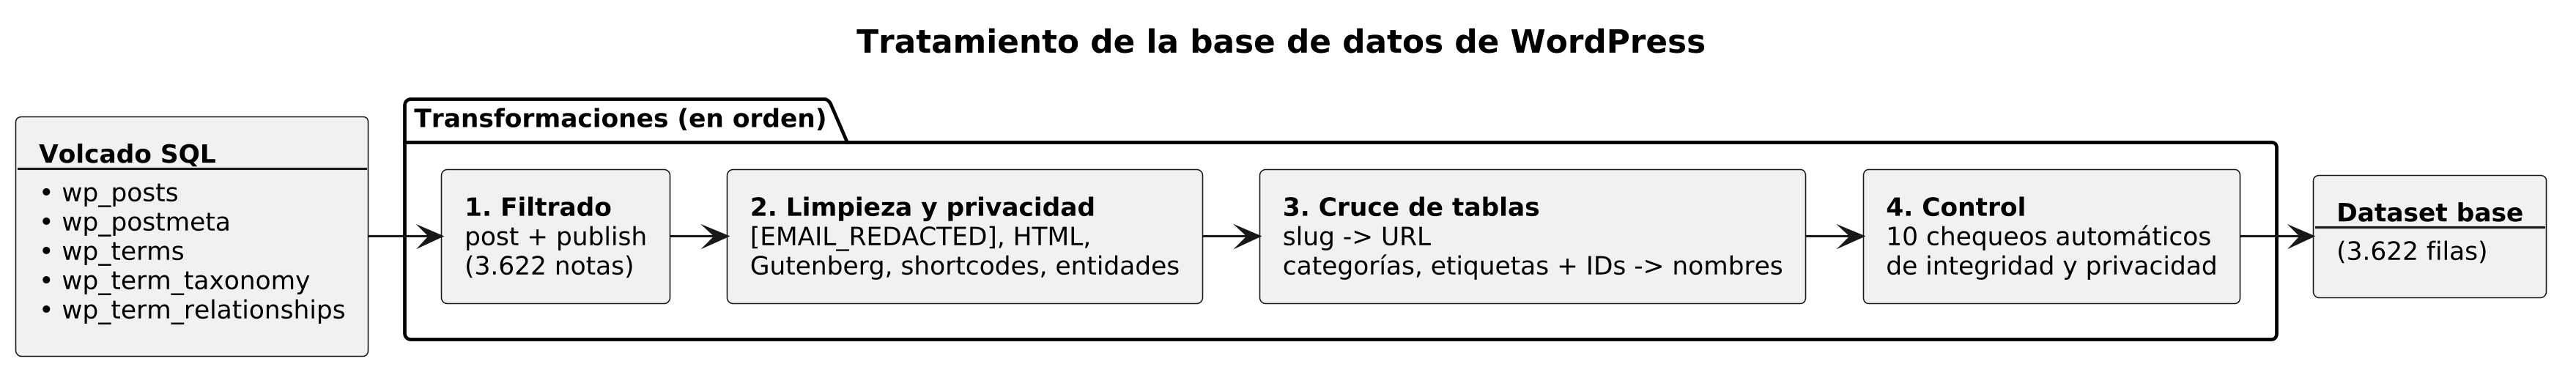
\includegraphics[keepaspectratio,alt={Procesamiento en
extract\_posteos\_anfibia.py}]{../docs/UML/2.1.1.png}}
\caption{Procesamiento en de la base de datos original}
\end{figure}

\paragraph{2.1.2. Exploración y Tratamiento de las
variables}\label{exploraciuxf3n-y-tratamiento-de-las-variables}

Una vez teniendo los artículos publicados, se exploraron las variables
elegidas y se realizaron otra ronda de operaciones de tratamiento:

\begin{itemize}
\item
  \textbf{Artículos sin cuerpo:} Se identificaron \textbf{26 artículos}
  con \texttt{body\_text} vacío. Al inspeccionar manualmente sus URLs,
  se verificó que correspondían a publicaciones multimedia (no artículos
  textuales) o solo contenían un título y un enlace de redirección hacia
  otra nota, por lo que fueron descartados.
\item
  \textbf{Diferentes versiones:} Cuando se republica o actualiza una
  nota, WordPress añade un sufijo numérico al \emph{slug} (\texttt{-2/},
  \texttt{-3/}, etc.). Se identificaron las notas que contaban con una
  versión posterior publicada y se excluyeron los originales
  reemplazados para evitar la duplicación de contenido.
\item
  \textbf{Idioma:} Mediante \texttt{langdetect} (aplicado sobre los
  primeros 500 caracteres de cada texto), se detectaron y excluyeron los
  artículos redactados en otros idiomas. Al revisarlos manualmente, se
  comprobó que los artículos clasificados como portugués (\texttt{pt})
  eran en realidad notas en español con citas o términos que confundían
  al detector, por lo que se conservaron.
\item
  \textbf{Integración:} Se consideró que tanto el \textbf{copete} (un
  anticipo breve sobre el tema de la nota) como el
  \textbf{\texttt{tagline}} (una frase de presentación) sintetizan la
  idea principal del artículo. Para que los modelos cuenten con la mayor
  información posible, en una primera instancia se evaluó concatenar
  únicamente el título y el cuerpo
  (\texttt{title\_text\ +\ ".\ "\ +\ body\_text}), pero finalmente se
  decidió incorporar también ambos campos cuando están presentes
  (\texttt{title\_text}, \texttt{copete}, \texttt{tagline} y
  \texttt{body\_text}), de modo que los modelos posteriores cuenten con
  mayor contexto semántico.
\end{itemize}

\begin{figure}[H]
\centering
\pandocbounded{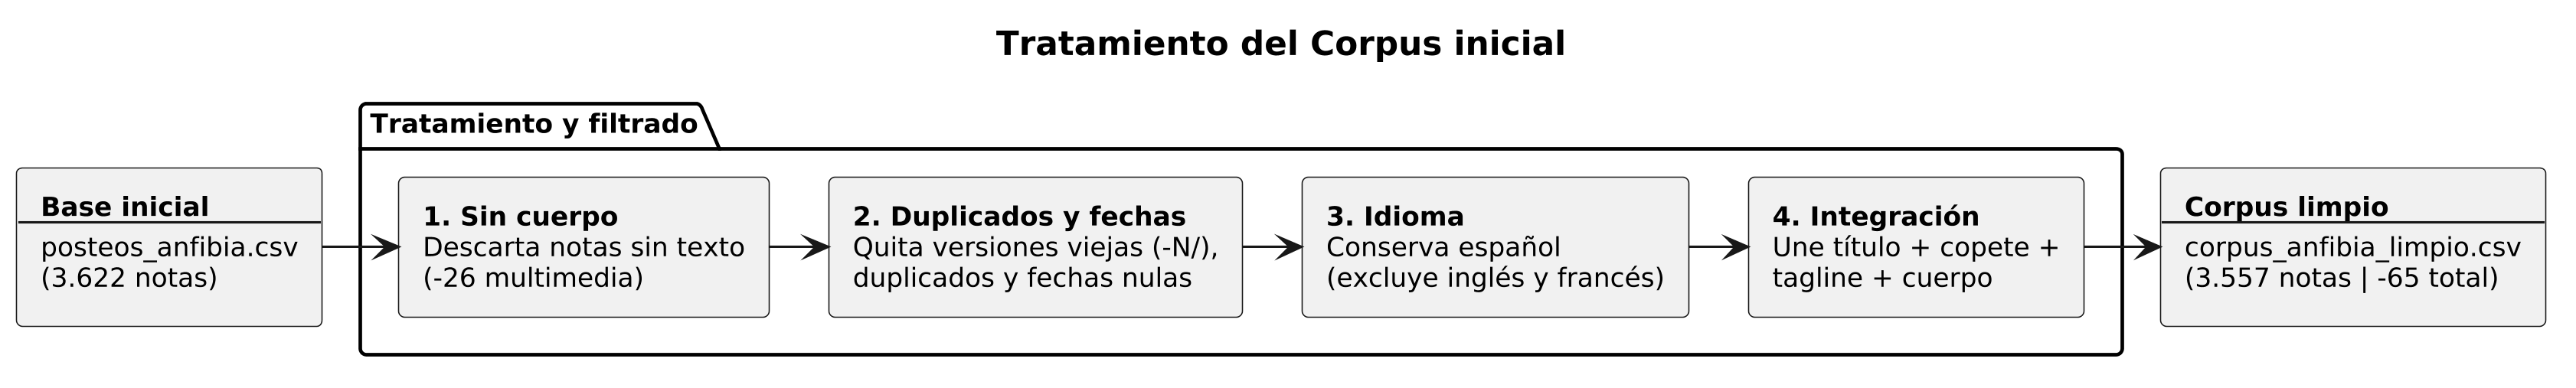
\includegraphics[keepaspectratio,alt={Tratamiento del
corpus inicial}]{../docs/UML/2.1.2.png}}
\caption{Tratamiento del corpus inicial}
\end{figure}

Y el corpus limpio consta de:

{\def\LTcaptype{none} % do not increment counter
\begin{longtable}[]{@{}
  >{\raggedright\arraybackslash}m{(\linewidth - 2\tabcolsep) * \real{0.5000}}
  >{\raggedright\arraybackslash}m{(\linewidth - 2\tabcolsep) * \real{0.5000}}@{}}
\toprule\noalign{}
\begin{minipage}[b]{\linewidth}\raggedright
Campo
\end{minipage} & \begin{minipage}[b]{\linewidth}\raggedright
Qué es
\end{minipage}\\ \midrule
\midrule\noalign{}
\endhead
\bottomrule\noalign{}
\endlastfoot
\textbf{\texttt{ID}} & Número único que identifica cada nota en la
base.\\ \midrule
\textbf{\texttt{title\_text}} & Título principal de la nota.\\ \midrule
\textbf{\texttt{copete}} & Anticipo corto que resume de qué va el
artículo antes de arrancar.\\ \midrule
\textbf{\texttt{tagline}} & Frase de presentación que acompaña al
título.\\ \midrule
\textbf{\texttt{body\_text}} & Cuerpo completo de la nota, ya limpio de
código HTML y bloques de WordPress.\\ \midrule
\textbf{\texttt{post\_name} / \texttt{source\_url}} & Identificador del
enlace y dirección pública de la nota
(\texttt{revistaanfibia.com/\textless{}post\_name\textgreater{}/}).\\ \midrule
\textbf{\texttt{post\_date}} & Fecha y hora de publicación de la
nota.\\ \midrule
\textbf{\texttt{category}} & Categoría del artículo (como \emph{Política
y Economía} o \emph{Culturas}).\\ \midrule
\textbf{\texttt{post\_tag}} & Etiquetas puestas a mano por los editores
para marcar temas puntuales.\\ \midrule
\textbf{\texttt{text\_type}} & Formato o género de la nota (crónica,
ensayo, perfil, entrevista, etc.).\\ \midrule
\textbf{\texttt{autor\_names} / \texttt{illustrator\_names}} & Nombres
de quienes escribieron e ilustraron el artículo.\\ \midrule
\textbf{\texttt{lang}} & Idioma detectado del texto en la etapa de
filtrado.\\ \midrule
\textbf{\texttt{document\_text\_extended}} & Texto unificado sumando
título, copete, tagline y cuerpo de la nota.\\ \midrule
\textbf{\texttt{word\_count\_extended}} & Cantidad de palabras del texto
unificado.\\ \midrule
\end{longtable}
}

\paragraph{2.1.3. Lematización y
stopwords}\label{lematizaciuxf3n-y-stopwords}

Los modelos posteriores (como las representaciones \emph{Bag-of-Words} y
la etapa de extracción de términos clave en Tópicos) dependen del conteo
y la frecuencia de las palabras dentro de los artículos. Dado que
originalmente contiene distintas variantes y plurales para un mismo
término (por ejemplo, contabilizando por separado \emph{elección} y
\emph{elecciones}, o \emph{calle} y \emph{calles}), se generó una
versión normalizada sin descartar el texto original, necesario para
otros aspectos (embeddings por ejemplo):

\begin{itemize}
\item
  \textbf{Lematización:} Se procesaron los artículos con el modelo en
  español \texttt{es\_core\_news\_md} de spaCy. Se conservaron
  únicamente palabras en minúscula reducidas a su lema base. Asimismo,
  se incorporó una regla manual para unificar \texttt{países} y
  \texttt{paises} en \texttt{país}, ya que el modelo los devolvía como
  lemas distintos. De este modo, el vocabulario resultante pasó de
  \textbf{\textasciitilde67.000} a \textbf{\textasciitilde43.000}
  términos.
\item
  \textbf{Stopwords:} Las \emph{stopwords} son palabras de muy alta
  frecuencia ---como artículos, preposiciones y conectores (\emph{el},
  \emph{de}, \emph{que}, \emph{para})--- que se filtran antes de
  analizar los textos porque aportan poco valor semántico y distorsionan
  las métricas de frecuencia. Al inspeccionar los términos más
  repetidos, también aparecieron palabras transversales a casi todas las
  notas sin importar los temas que tratan ---como \emph{anfibia},
  \emph{revista}, \emph{crónica}, \emph{argentina}, \emph{país},
  \emph{político}, \emph{tiempo}, \emph{vida} o \emph{persona}---, por
  lo que se construyó un diccionario propio de \emph{stopwords} de
  dominio para utilizar en el modelado temático.
\end{itemize}

\emph{(Nota: Este listado de Stopwords se amplió iterativamente al
analizar los términos clave de los tópicos, como se detallará en la
sección correspondiente).}

\begin{itemize}
\tightlist
\item
  \textbf{Algunos Resultados:}
\end{itemize}

Al comparar las 10 palabras más frecuentes antes y después de la
lematización (filtrando únicamente las \emph{stopwords} básicas del
español), se observa cómo variantes que antes quedaban repartidas se
concentran en un único lema: por ejemplo, \emph{social} (6.805) y
\emph{sociales} (5.719) se unifican en \emph{social} (12.229), y
\emph{mujeres} se agrupa bajo \emph{mujer} (10.692).

% \textbf{Sin lematizar}

% {\def\LTcaptype{none} % do not increment counter
% \begin{longtable}[]{@{}lcc@{}}
% \toprule\noalign{}
% Palabra & Artículos & Frecuencia total\\ \midrule
% \midrule\noalign{}
% \endhead
% \bottomrule\noalign{}
% \endlastfoot
% \emph{puede} & 2.761 & 9.296\\ \midrule
% \emph{gobierno} & 1.755 & 8.274\\ \midrule
% \emph{mundo} & 2.451 & 8.239\\ \midrule
% \emph{pais} & 2.205 & 7.423\\ \midrule
% \emph{mujeres} & 1.445 & 7.370\\ \midrule
% \emph{trabajo} & 2.157 & 7.205\\ \midrule
% \emph{personas} & 2.173 & 6.837\\ \midrule
% \emph{social} & 2.069 & 6.805\\ \midrule
% \emph{casa} & 1.850 & 6.767\\ \midrule
% \emph{sociales} & 1.944 & 5.719\\ \midrule
% \ldots{} & \ldots{} & \ldots{}\\ \midrule
% \end{longtable}
% }

% \textbf{Lematizado}

% {\def\LTcaptype{none} % do not increment counter
% \begin{longtable}[]{@{}lcc@{}}
% \toprule\noalign{}
% Palabra & Artículos & Frecuencia total\\ \midrule
% \midrule\noalign{}
% \endhead
% \bottomrule\noalign{}
% \endlastfoot
% \emph{politico} & 2.269 & 12.372\\ \midrule
% \emph{social} & 2.536 & 12.229\\ \midrule
% \emph{mujer} & 1.884 & 10.692\\ \midrule
% \emph{pais} & 2.417 & 9.843\\ \midrule
% \emph{politica} & 2.138 & 9.611\\ \midrule
% \emph{gobierno} & 1.859 & 9.327\\ \midrule
% \emph{publico} & 2.386 & 8.656\\ \midrule
% \emph{mundo} & 2.477 & 8.512\\ \midrule
% \emph{casa} & 2.009 & 7.963\\ \midrule
% \emph{trabajo} & 2.182 & 7.376\\ \midrule
% \ldots{} & \ldots{} & \ldots{}\\ \midrule
% \end{longtable}
% }

\begin{table}[H]
\centering
\begin{minipage}[t]{0.48\linewidth}
\centering
\textbf{Sin lematizar}\\[6pt]
\begin{tabular}{@{}lcc@{}}
\toprule
Palabra & Artículos & Frecuencia total \\
\midrule
\emph{puede} & 2.761 & 9.296 \\ \midrule
\emph{gobierno} & 1.755 & 8.274 \\ \midrule
\emph{mundo} & 2.451 & 8.239 \\ \midrule
\emph{pais} & 2.205 & 7.423 \\ \midrule
\emph{mujeres} & 1.445 & 7.370 \\ \midrule
\emph{trabajo} & 2.157 & 7.205 \\ \midrule
\emph{personas} & 2.173 & 6.837 \\ \midrule
\emph{social} & 2.069 & 6.805 \\ \midrule
\emph{casa} & 1.850 & 6.767 \\ \midrule
\emph{sociales} & 1.944 & 5.719 \\ \midrule
\ldots{} & \ldots{} & \ldots{} \\
\bottomrule
\end{tabular}
\end{minipage}
\hfill
\begin{minipage}[t]{0.48\linewidth}
\centering
\textbf{Lematizado}\\[6pt]
\begin{tabular}{@{}lcc@{}}
\toprule
Palabra & Artículos & Frecuencia total \\
\midrule
\emph{politico} & 2.269 & 12.372 \\ \midrule
\emph{social} & 2.536 & 12.229 \\ \midrule
\emph{mujer} & 1.884 & 10.692 \\ \midrule
\emph{pais} & 2.417 & 9.843 \\ \midrule
\emph{politica} & 2.138 & 9.611 \\ \midrule
\emph{gobierno} & 1.859 & 9.327 \\ \midrule
\emph{publico} & 2.386 & 8.656 \\ \midrule
\emph{mundo} & 2.477 & 8.512 \\ \midrule
\emph{casa} & 2.009 & 7.963 \\ \midrule
\emph{trabajo} & 2.182 & 7.376 \\ \midrule
\ldots{} & \ldots{} & \ldots{} \\
\bottomrule
\end{tabular}
\end{minipage}
\end{table}

\emph{Nota: Mientras que la frecuencia total suma las apariciones individuales en todo el archivo, el conteo de artículos refleja la cantidad de notas distintas donde el lema aparece al menos una vez; dado que muchos artículos emplean tanto el singular como el plural en un mismo texto (por ejemplo, \emph{social} y \emph{sociales}), al unificarse se contabilizan una única vez.}

A modo de ejemplo visual, se compara la nube de palabras (cada palabra
tiene un tamaño proporcional a su frecuencia) para la categoría
\textbf{Política y Economía} antes y después de aplicar la lematización:

\textbf{Sin lematizar}

\begin{figure}[H]
\centering
\pandocbounded{\includegraphics[keepaspectratio,alt={Nube sin lematizar
--- Política y
Economía}]{../outputs/figuras_informe/wordcloud_politica_sin_lematizar.png}}
\caption{Nube sin lematizar --- Política y Economía}
\end{figure}

\textbf{Lematizado}

\begin{figure}[H]
\centering
\pandocbounded{\includegraphics[keepaspectratio,alt={Nube lematizada ---
Política y
Economía}]{../outputs/wordclouds_by_category_lematizado/wordcloud_politica-y-economia.png}}
\caption{Nube lematizada --- Política y Economía}
\end{figure}

En esta comparación se observa cómo en la versión sin lematizar ocupan
un lugar central verbos y palabras de poco aporte (\emph{puede},
\emph{sido}, \emph{hizo}, \emph{quienes}, \emph{estas}, \emph{todas}),
además de aparecer dispersas diferentes variantes (\emph{social} /
\emph{sociales}). En la nube lematizada, en cambio, desaparecen esas
palabras vacías y se concentran en sus lemas.

\subsubsection{2.2. Modelado de tópicos}\label{modelado-de-tuxf3picos}

El objetivo del modelado de tópicos es descubrir los núcleos temáticos
reales alrededor de los cuales se concentran los artículos, sin depender
de una asignación manual. Contar con ellos permite analizar cómo
evolucionó \emph{Revista Anfibia} a lo largo de los años y establecer
una base sobre la cual desarrollar un sistema de recomendación por
similitud temática.

\paragraph{2.2.1. Tópicos con BerTopic}\label{tuxf3picos-con-bertopic}

Antes de llegar a este modelo, se probaron otros enfoques basados
únicamente en conteo de palabras (como LDA) y modelos de
\emph{embeddings} en español. El problema de usar solo el conteo de
palabras es que dos artículos sobre el mismo tema pueden usar
vocabularios muy distintos, por lo que se descartó LDA. Por otro lado,
si se usan únicamente \emph{embeddings} (agrupando notas), se consiguen
tópicos coherentes pero el modelo no devuelve por sí solo una manera de
explicar de qué trata cada uno.

Por eso se recurrió a \textbf{BERTopic}, que además de la creación de
tópicos nos proporciona la extracción de palabras clave y otras
funcionalidades. En esta primera etapa, para detectar los Tópicos se
calcularon \emph{embeddings} (embeddings, ver Anexo A.1) sobre el texto
original sin lematizar usando el modelo
\texttt{paraphrase-multilingual-MiniLM-L12-v2}, de manera que tiene en
cuenta la estructura de las oraciones y el contexto de las palabras en
ellas, algo que se pierde con la lematización. Como cada artículo queda
representado en un espacio de 384 dimensiones (sus embeddings), primero
se comprimieron esos vectores con \texttt{UMAP} conservando tanto la
cercanía entre notas parecidas como la estructura general.

Sobre ese espacio reducido se aplicó el algoritmo de agrupamiento por
densidad \texttt{HDBSCAN} (\texttt{min\_cluster\_size=10},
\texttt{min\_samples=3}). A diferencia de otros métodos que exigen fijar
de antemano cuántos tópicos existen y obligan a meter cada artículo en
alguno aunque no encaje, \texttt{HDBSCAN} busca zonas donde se acumula
una alta densidad de artículos similares entre sí, permitiendo que cada
tópico decida sus artículos. Además, deja un tópico aparte (\texttt{-1})
todas las notas demasiado específicas que no encajan claramente en
ningún Tópico; esto evita contaminar los principales y mejora la calidad
de las palabras clave extraídas para cada tópico.

Con esos parámetros se buscó que el modelo identifique Tópicos muy
definidos aunque no lleguen a tener un gran número de notas.

\emph{Nota: La asignación principal de cada artículo surge del agrupamiento por densidad 
en el espacio de embeddings (y de la posterior reasignación por umbral, donde 
se le asigna su tópico más similar o queda como outlier en el Tópico 100).}

\begin{figure}[H]
\centering
\pandocbounded{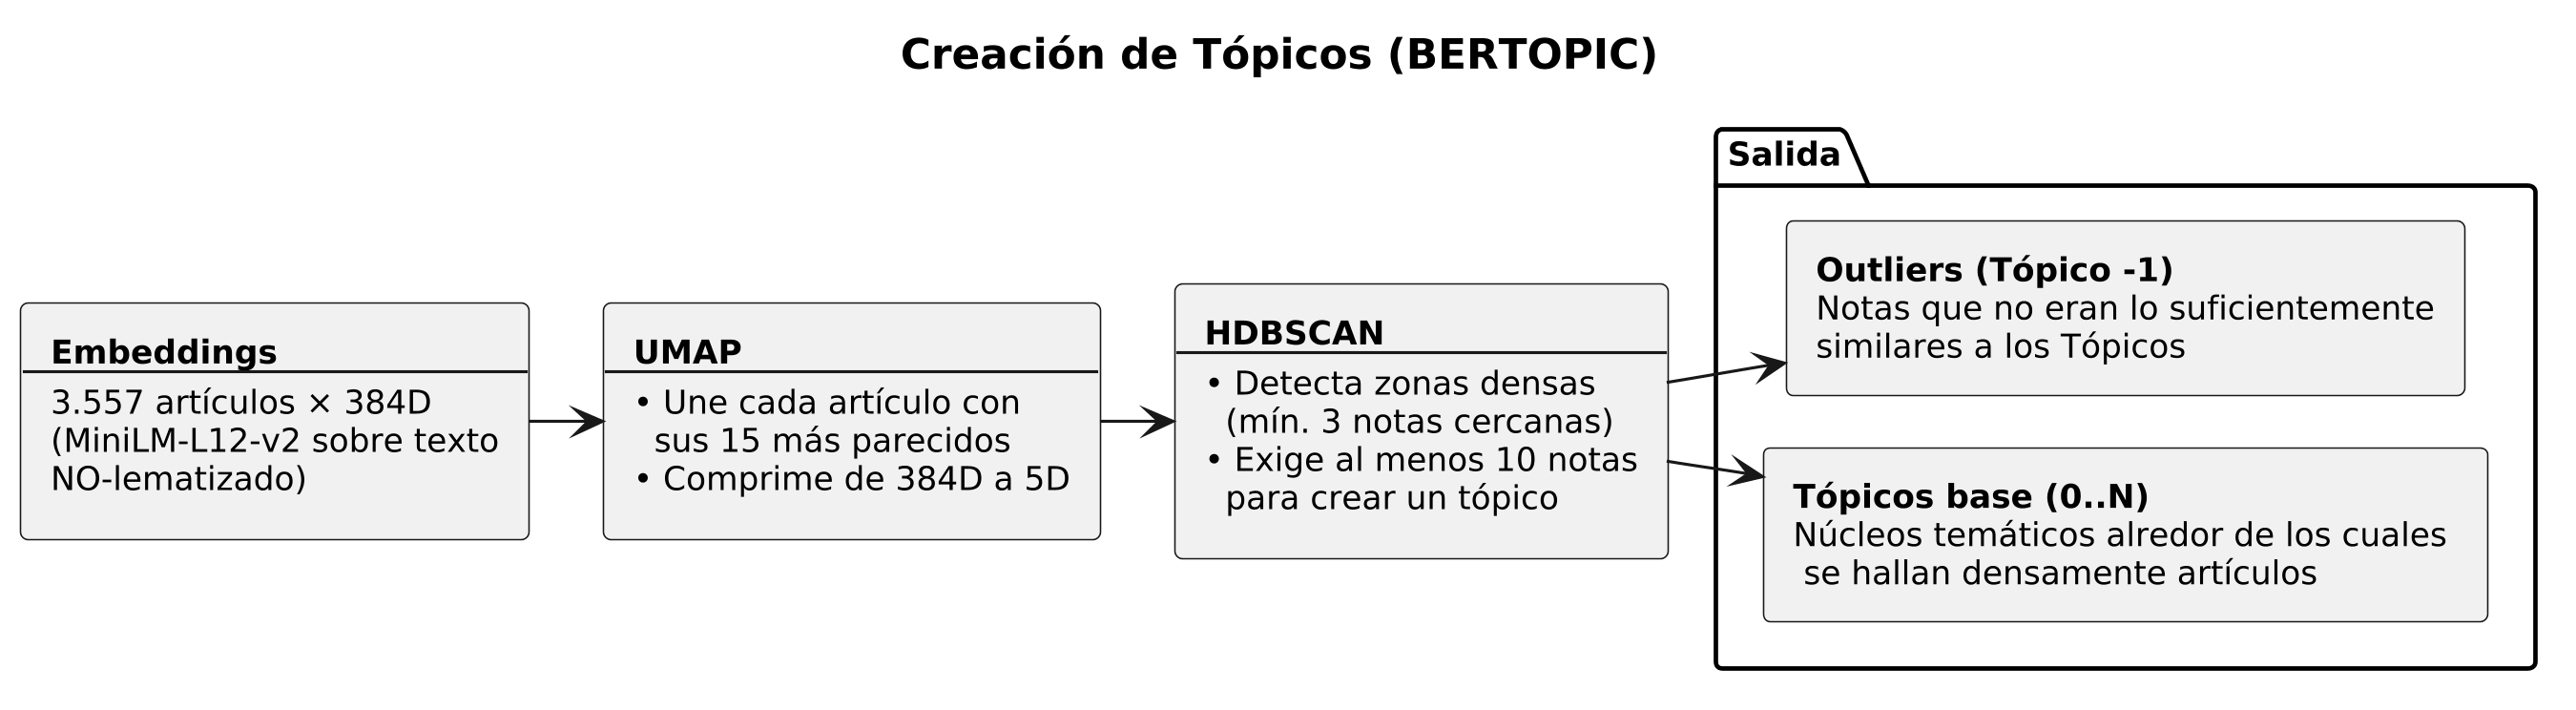
\includegraphics[keepaspectratio]{../docs/UML/2.2.1.png}}
\caption{Diagrama del pipeline de modelado de tópicos con BERTopic}
\end{figure}

\paragraph{2.2.2. Palabras clave de cada
tópico}\label{palabras-clave-de-cada-tuxf3pico}

\textbf{Creación}

Una vez formados los tópicos (que inicialmente solo cuentan con un
identificador numérico), el siguiente paso fue asignarles un nombre que
refleje las notas que representan. Se optó por no redactar nombres
manualmente para evitar errores de interpretación o sesgos, aun habiendo
leído una muestra de los artículos de cada uno.

Aquí entra en juego otra funcionalidad de BERTopic: la extracción
automática de palabras clave para cada tópico, de modo que su nombre
quede definido por sus propios términos más representativos. Para
calcular qué términos definen mejor a cada núcleo, primero BERTopic
concatena todos los artículos asignados a un mismo tópico como si fueran
un único documento y aplica \textbf{c-TF-IDF} (\emph{Class-based
TF-IDF}). Mientras que el TF-IDF clásico mide qué tan importante es una
palabra dentro de un artículo frente al resto del corpus,
\texttt{c-TF-IDF} mide qué tan importante es una palabra dentro de un
tópico frente a los demás. De este modo, las palabras transversales (en
varios tópicos) pierden peso y ganan relevancia aquellas que distinguen
específicamente a cada tópico.

Sin embargo, quedarse únicamente con los puntajes más altos de
\texttt{c-TF-IDF} presenta una limitación: en ocasiones premia términos
muy puntuales que se repitieron con frecuencia en una o dos crónicas
extensas, pero que no representan al resto de los artículos del núcleo.
Para resolverlo, se agregó \textbf{\texttt{KeyBERTInspired}}, un paso
que toma las mejores palabras candidatas de \texttt{c-TF-IDF}, calcula
sus \emph{embeddings} y mide su cercanía con respecto al centroide
(centroide, ver Anexo A.2) de todo el tópico. Así, las palabras clave
finales no solo son frecuentes dentro de ese núcleo y poco habituales en
los demás, sino que reflejan el sentido global de todos los artículos
que lo integran.

\begin{figure}[H]
\centering
\pandocbounded{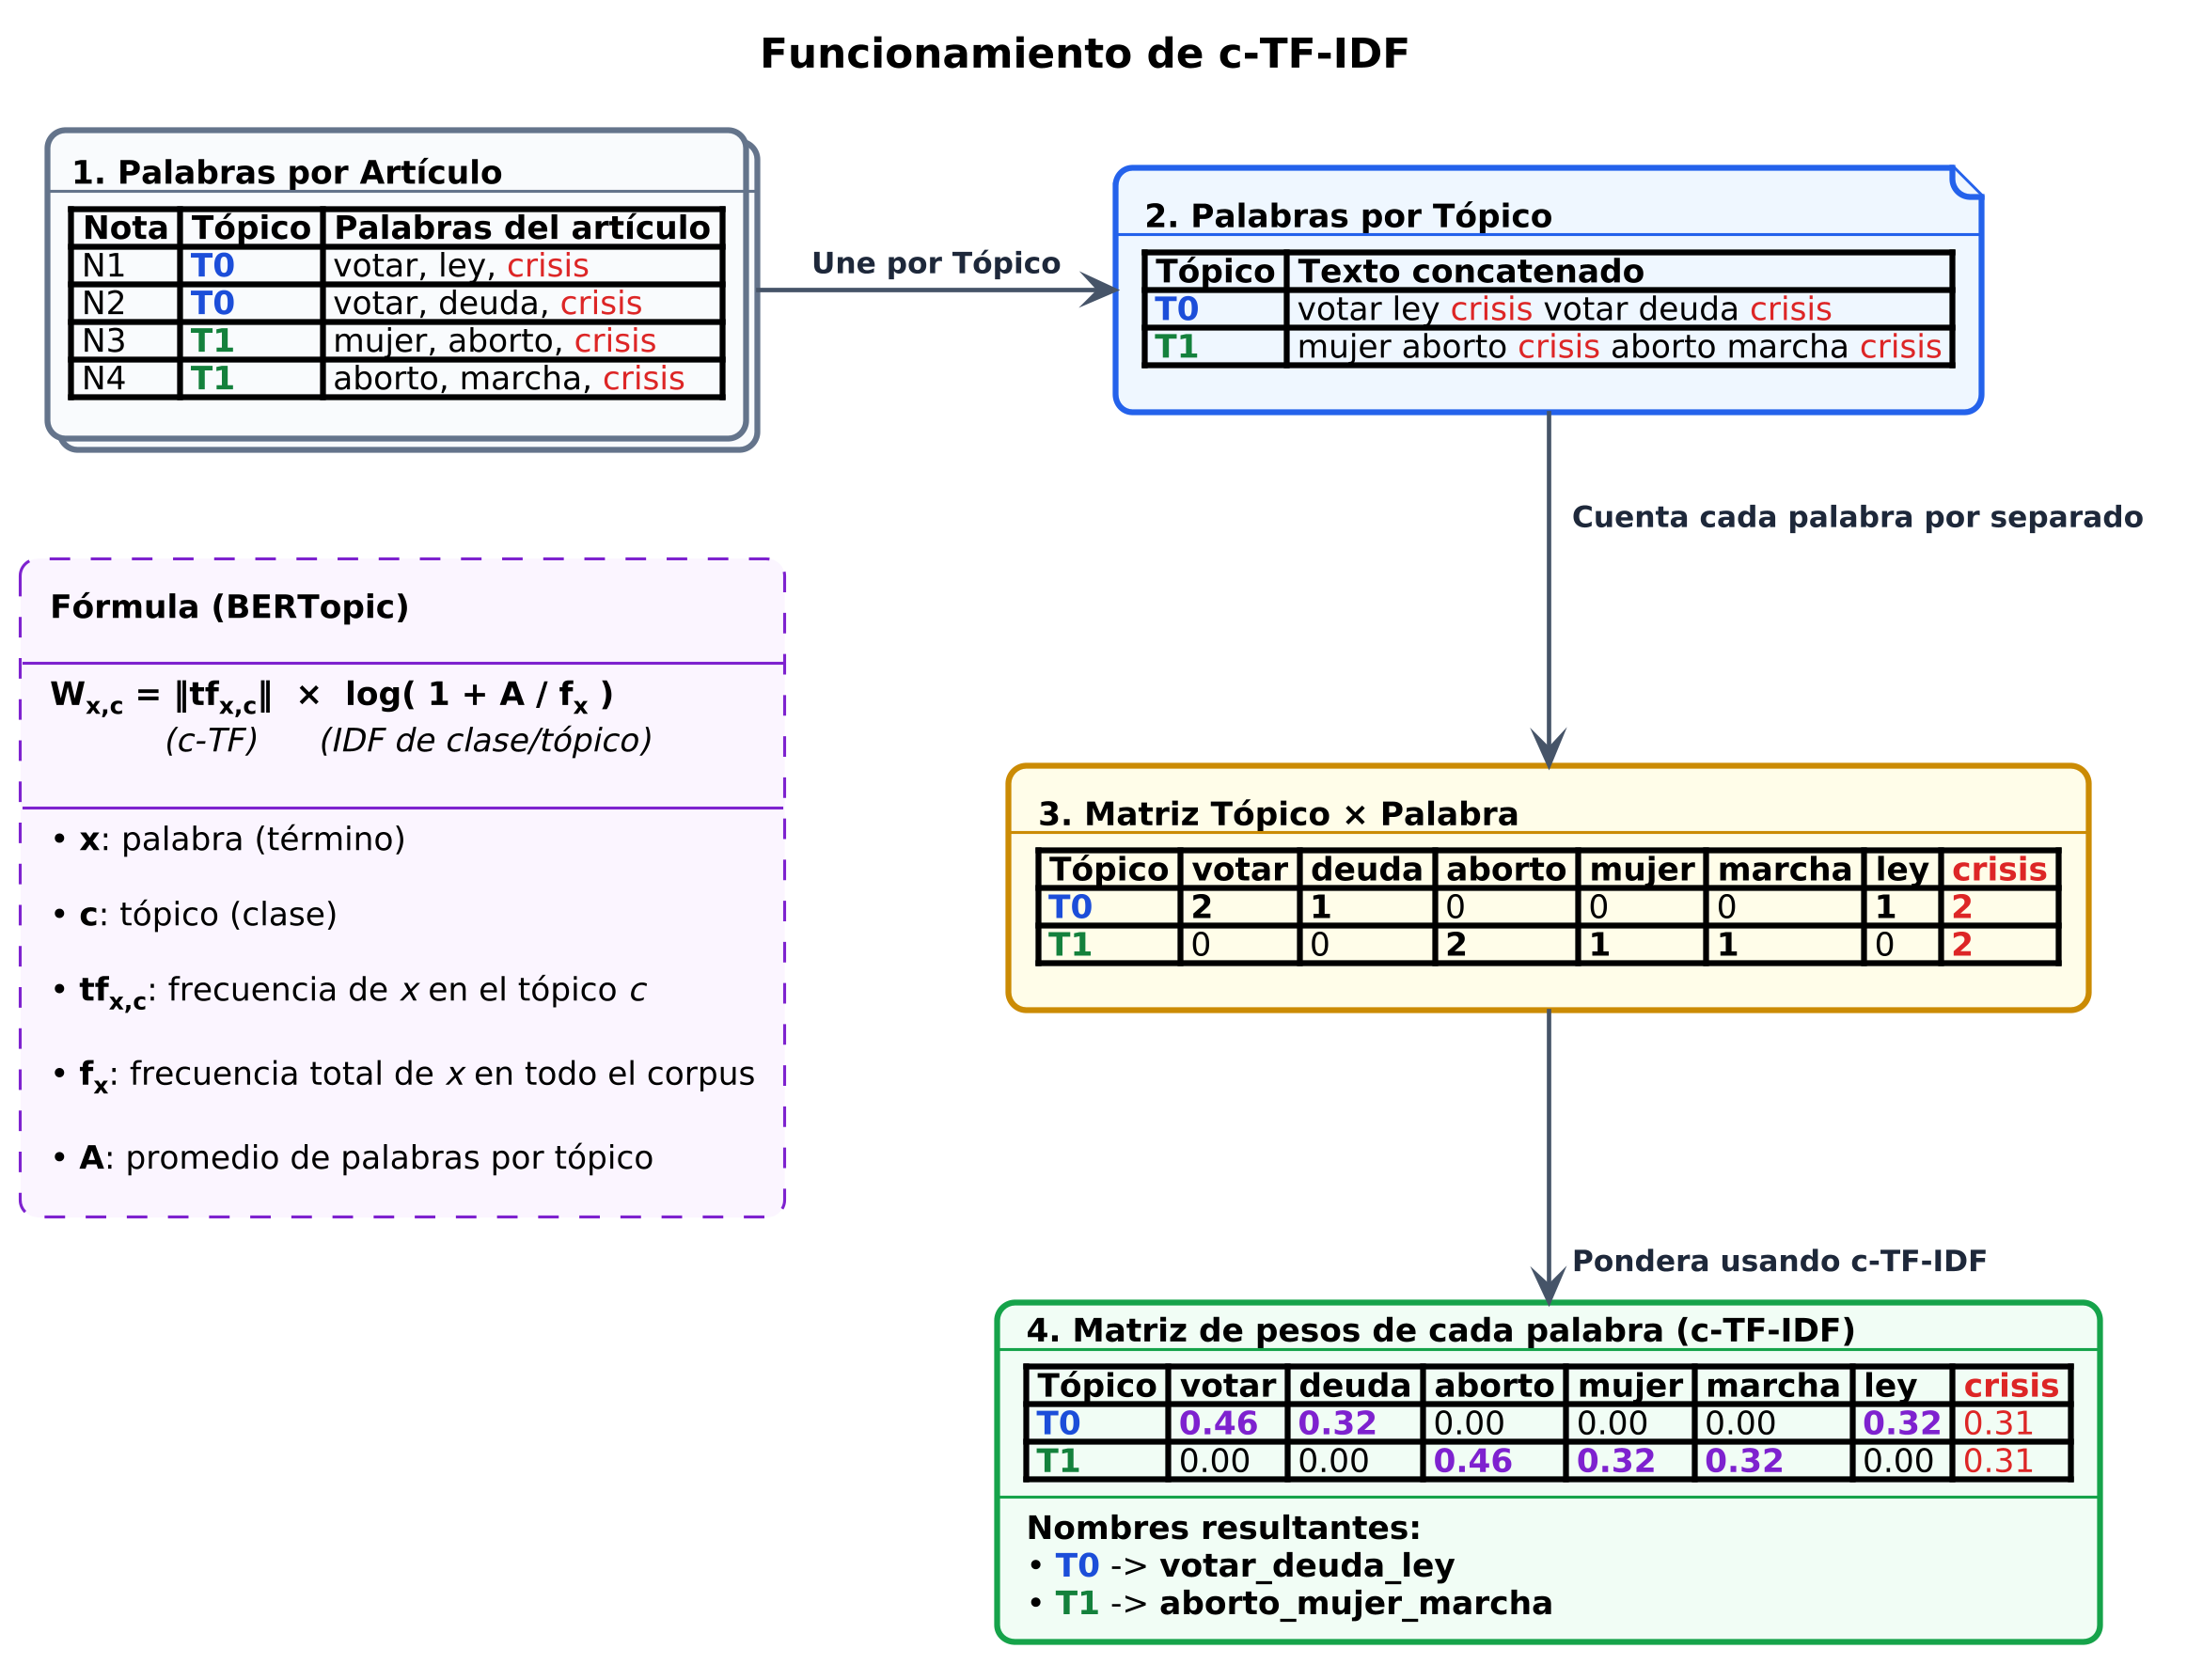
\includegraphics[keepaspectratio]{../docs/UML/2.2.2.png}}
\caption{Diagrama del cálculo de c-TF-IDF}
\end{figure}

En el ejemplo, dividir la cantidad de veces que aparece cada palabra por
el total de palabras del tópico (\(\Vert{}tf_{x,c}\Vert{}\)) sirve para
trabajar con proporciones y compensar que un tópico tenga muchas más
notas que otro. Por su parte, el logaritmo baja el puntaje de las
palabras que aparecen repetidas por todo el archivo (\(f_x\)) frente al
promedio de palabras por tópico (\(A\)). En el diagrama se ve bien qué
pasa con la palabra en rojo (\emph{crisis}): como aparece en notas de
ambos tópicos (\texttt{N1} a \texttt{N4}), en el conteo suma \textbf{2}
apariciones tanto en \texttt{T0} como en \texttt{T1}, empatando con las
palabras propias de cada uno (\emph{votar} en \texttt{T0} y
\emph{aborto} en \texttt{T1}). Pero al aplicar \texttt{c-TF-IDF}, como
\emph{crisis} está en ambos (\(f_x = 4\)), el cálculo la penaliza y su
puntaje cae a \textbf{\texttt{0.31}} en los dos tópicos, mientras que
las palabras que sí son exclusivas de cada tema quedan arriba con
\textbf{\texttt{0.46}} y \textbf{\texttt{0.32}}. De esta manera,
\emph{crisis} queda afuera y los nombres se arman solo con los términos
que realmente distinguen a cada tópico (\texttt{votar\_deuda\_ley} para
\texttt{T0} y \texttt{aborto\_mujer\_marcha} para \texttt{T1}).

\textbf{Uso en la iteración de Stopwords}

Al revisar las primeras listas de palabras clave de cada tópico (en esta
etapa todavía no se habían generado nubes de palabras por tópico, sino
que se inspeccionaban directamente mediante gráficos de barras con los
puntajes de relevancia), surgió un problema: aparecían términos con alto
peso en varios núcleos simultáneamente que, aun teniendo un puntaje
\texttt{c-TF-IDF} elevado, dificultaban interpretar de qué trataba cada
tópico.

Para corregir esto se hizo un proceso iterativo: se revisaban los
rankings de palabras de cada tópico, se anotaban los términos relevantes
pero que abarcaban varios tópicos o no tenían importancia y se los
agregaba en tandas sucesivas a las stopwords, cuidando de dejar afuera
palabras que sí representen individualidad de los Tópicos.

La comparación de los 6 tópicos con mayor volumen del modelo antes y
después de ampliar las Stopwords muestra cómo este filtrado aclara que
significa cada Tópico:

{\def\LTcaptype{none} % do not increment counter
\begin{longtable}[]{@{}
  >{\raggedright\arraybackslash}m{(\linewidth - 4\tabcolsep) * \real{0.3333}}
  >{\raggedright\arraybackslash}m{(\linewidth - 4\tabcolsep) * \real{0.3333}}
  >{\raggedright\arraybackslash}m{(\linewidth - 4\tabcolsep) * \real{0.3333}}@{}}
\toprule\noalign{}
\begin{minipage}[b]{\linewidth}\raggedright
Tópico
\end{minipage} & \begin{minipage}[b]{\linewidth}\raggedright
Palabras clave antes (Stopwords generales)
\end{minipage} & \begin{minipage}[b]{\linewidth}\raggedright
Palabras clave después (agregando Stopwords)
\end{minipage}\\ \midrule
\midrule\noalign{}
\endhead
\bottomrule\noalign{}
\endlastfoot
\textbf{Tópico 00} & \emph{político, política, candidato, electoral,
campaña, votar} & \emph{candidato, electoral, campaña, debate, votar,
discurso}\\ \midrule
\textbf{Tópico 01} & \emph{autor, escritor, literatura, novela,
personaje, libro} & \emph{literario, autor, escritor, poeta,
protagonista, literatura}\\ \midrule
\textbf{Tópico 02} & \emph{feminismo, feminista, aborto, político,
política, debate} & \emph{feminismo, feminista, aborto, abortar,
patriarcado, debate}\\ \midrule
\textbf{Tópico 03} & \emph{historia, vivir, hombre, vida, muerte,
contar} & \emph{muerto, dictadura, muerte, morir, desaparición, cuba}\\ \midrule
\textbf{Tópico 04} & \emph{político, política, cambio, decir, además,
seguir} & \emph{ambiental, ambiente, crisis, proyecto, sociedad,
futuro}\\ \midrule
\textbf{Tópico 05} & \emph{economía, crisis, pobreza, económico,
reforma, inflación} & \emph{déficit, economía, pobreza, económico,
fiscal, deuda}\\ \midrule
\end{longtable}
}

Se nota en los tópicos \textbf{03} y \textbf{04}: el primero pasa de
términos más genéricos (\emph{historia, vivir, hombre, vida}) a reflejar
temáticas de memoria y dictadura, mientras que el segundo quita las
palabras comúnes o sin importancia (\emph{político, decir, además}) y
revela una temática ambiental.

\emph{(Nota: Esta última tabla se generó utilizando el modelo final ya
consolidado, por lo que la numeración de los tópicos no coincide
exactamente con la del modelo preliminar sobre el cual se realizó la
iteración de stopwords).}

\paragraph{2.2.3. Reducción y fusión iterativa de
tópicos}\label{reducciuxf3n-y-fusiuxf3n-iterativa-de-tuxf3picos}

Al generar los tópicos iniciales, se dejó que el modelo tuviera libertad
para crear Tópicos y lograr así alta granularidad, de modo que cada uno
conservara un significado específico. Sin embargo, el total resultante
fue demasiado elevado (\textbf{79 tópicos activos}), lo que dificultaba
la lectura general y los análisis siguientes.

Si se aplica una reducción automática (\texttt{nr\_topics=\textquotedbl{}auto\textquotedbl{}}),
BERTopic fusiona núcleos según umbrales internos y suele mezclar temas
distintos (por ejemplo, un tópico sobre procesos electorales con otro
sobre macroeconomía, simplemente porque comparten vocabulario). Por
ello, se optó por una estrategia en dos etapas: aplicar primero una
reducción automática moderada hasta \textbf{40 tópicos activos} y luego
evaluar manualmente los restantes para decidir cuáles unir.

Para decidir qué tópicos unir se utilizó
\textbf{\texttt{visualize\_hierarchy}}, una herramienta de BERTopic que
aplica \textbf{clustering jerárquico aglomerativo} entre las
representaciones \texttt{c-TF-IDF} de cada tópico. El resultado es un
dendrograma donde la longitud de cada rama indica qué tan distintos son
dos tópicos en términos sus palabras: las ramas que se unen más cerca de
la base (menor distancia) son las que BERTOPIC considera candidatas a
unirse.

De este modo, se iteró aplicando dos verificaciones antes de ejecutar
\textbf{\texttt{merge\_topics()}} (función que unifica los documentos de
los tópicos seleccionados y recalcula sus palabras clave):

\begin{enumerate}
\def\labelenumi{\arabic{enumi}.}
\item
  \textbf{Lectura del dendrograma:} Identificación de pares de Tópicos
  de ramas con menor distancia del coseno (sim. y dist. coseno, ver
  Anexo A.3) entre sus vectores \texttt{c-TF-IDF}.
\item
  \textbf{Inspección de palabras clave:} Verificación de que los
  términos principales de ambos tópicos realmente tienen una tematica
  similar y no a fenómenos distintos que utilizan palabras similares.
\end{enumerate}

Finalmente se realizaron 4 iteraciones:

% {\def\LTcaptype{none} % do not increment counter
% \begin{longtable}[]{@{}ll@{}}
% \toprule\noalign{}
% Etapa & Cantidad de tópicos\\ \midrule
% \midrule\noalign{}
% \endhead
% \bottomrule\noalign{}
% \endlastfoot
% \textbf{Modelo Inicial} & 79\\ \midrule
% \textbf{1.ª fusión (automática)} & \textbf{40}\\ \midrule
% \textbf{2.ª fusión} & \textbf{30}\\ \midrule
% \textbf{3.ª fusión} & \textbf{27}\\ \midrule
% \textbf{4.ª fusión (final)} & \textbf{22}\\ \midrule
% \end{longtable}
% }

\begin{center}
\begin{tabular}{@{}lc@{}}
\toprule
Etapa & Cantidad de tópicos \\
\midrule
\textbf{Modelo Inicial} & 79 \\ \midrule
\textbf{1.\textsuperscript{a} fusión (automática)} & \textbf{40} \\ \midrule
\textbf{2.\textsuperscript{a} fusión} & \textbf{30} \\ \midrule
\textbf{3.\textsuperscript{a} fusión} & \textbf{27} \\ \midrule
\textbf{4.\textsuperscript{a} fusión (final)} & \textbf{22} \\
\bottomrule
\end{tabular}
\end{center}

El proceso se detuvo en la 4ta fusión, al inspeccionar el dendrograma,
las siguientes uniones implicaban distancias del coseno demasiado
elevadas. Continuar habría unido Tópicos conceptualmente distantes,
perdiendo la especificidad alcanzada.

\emph{(Nota: Si bien se fijó \texttt{random\_state=42} en UMAP, el
agrupamiento por densidad de HDBSCAN puede alterar la numeración interna
de los tópicos iniciales (\texttt{0..N}). Como las fusiones guiadas se
aplican sobre los IDs específicos generados en esta ejecución, el modelo
final no es estrictamente reproducible, al menos sin modificar el código
existente).}

\begin{figure}[H]
\centering
\pandocbounded{\includegraphics[keepaspectratio,alt={Dendrograma de
jerarquía de los 22
tópicos}]{../outputs/figuras_informe/dendrograma_topicos_final.png}}
\caption{Dendrograma de jerarquía de los 22 tópicos}
\end{figure}

Incluso en los pares con menor distancia coseno dentro de ese árbol
final, la cercanía responde al uso similar de palabras, pero cada tópico
mantiene una identidad propia que se perdería al consolidarlos. Por
ejemplo, aunque los tópicos \textbf{04} y \textbf{05} aparecen próximos
en el dendrograma, al revisar los títulos y \emph{taglines} de sus
artículos se comprueba que abordan fenómenos diferenciados:

\begin{itemize}
\tightlist
\item
  \textbf{Tópico 04 (\texttt{4\_ambiental\_ambiente\_crisis}):} Temas
  territoriales, productivos y socioambientales.

  \begin{itemize}
  \tightlist
  \item
    \emph{``La reforma agraria de las mujeres guaraníes''}
  \item
    \emph{``Epecuén jamás se inundaría''} --- \emph{Tagline: Adelanto}
  \item
    \emph{``Copiapó: si la luz fuera líquida''} --- \emph{Tagline:
    Adelanto}
  \end{itemize}
\item
  \textbf{Tópico 05 (\texttt{5\_déficit\_economía\_pobreza}):} Análisis
  financieros, cambiarios y macroeconómicos.

  \begin{itemize}
  \tightlist
  \item
    \emph{``Todo sobre los buitres''} --- \emph{Tagline: Deuda externa}
  \item
    \emph{``DÓLAR BLUE: LA CORRIDA QUE NO FUE''} --- \emph{Tagline:
    Mercados}
  \item
    \emph{``Syriza: golpear y negociar''} --- \emph{Tagline: Crisis
    europea}
  \end{itemize}
\end{itemize}

\paragraph{\texorpdfstring{2.2.4. Tratamiento de \emph{outliers}
(\texttt{Tópico\ -1})}{2.2.4. Tratamiento de outliers (Tópico -1)}}\label{tratamiento-de-outliers-tuxf3pico--1}

Una proporción importante de los artículos quedó inicialmente sin
asignación temática bajo la etiqueta \texttt{-1} (\emph{outliers}). Se
evaluaron dos estrategias para integrar parte de estos documentos sin
degradar la calidad de los 22 tópicos consolidados:

\begin{enumerate}
\def\labelenumi{\arabic{enumi}.}
\tightlist
\item
  \textbf{Reasignación forzada :} Asigna el 100 \% de los \texttt{-1} al
  tópico con el centroide más cercano. Si bien elimina por completo los
  \emph{outliers}, diluye las palabras clave (\texttt{c-TF-IDF}) y
  reduce la coherencia de los Tópicos.
\item
  \textbf{Reasignación acotada por umbral de similitud coseno
  (\(\ge 0,65\)):} Se calculó el centroide semántico de cada uno de los
  22 tópicos promediando los \emph{embeddings} naturales (texto sin
  lematizar) de sus artículos. Luego se midió la similitud del coseno
  entre cada documento \texttt{-1} y los 22 centroides, reasignando
  únicamente aquellas notas cuya similitud máxima alcanzara o superara
  \texttt{0,65}, y por último se recalibraron los pesos c-TF-IDF.
\end{enumerate}

Se decidió optar por la segunda opción. Lo cual redujo los Outliers:

\begin{figure}[H]
\centering
\pandocbounded{\includegraphics[keepaspectratio,alt={Proporción de
artículos asignados frente a outliers antes y después del
umbral}]{../outputs/figuras_informe/proporcion_outliers.png}}
\caption{Proporción de artículos asignados frente a outliers antes y
después del umbral}
\end{figure}

Con ello, los Tópicos finales son:

{\def\LTcaptype{none} % do not increment counter
\begin{longtable}[]{@{}
  >{\raggedright\arraybackslash}m{(\linewidth - 8\tabcolsep) * \real{0.1739}}
  >{\raggedright\arraybackslash}m{(\linewidth - 8\tabcolsep) * \real{0.1739}}
  >{\centering\arraybackslash}m{(\linewidth - 8\tabcolsep) * \real{0.2174}}
  >{\centering\arraybackslash}m{(\linewidth - 8\tabcolsep) * \real{0.2174}}
  >{\centering\arraybackslash}m{(\linewidth - 8\tabcolsep) * \real{0.2174}}@{}}
\toprule\noalign{}
\begin{minipage}[b]{\linewidth}\raggedright
Tópico
\end{minipage} & \begin{minipage}[b]{\linewidth}\raggedright
Palabras clave principales
\end{minipage} & \begin{minipage}[b]{\linewidth}\centering
Artículos (base)
\end{minipage} & \begin{minipage}[b]{\linewidth}\centering
Artículos (umbral \(\ge 0,65\))
\end{minipage} & \begin{minipage}[b]{\linewidth}\centering
Variación
\end{minipage}\\ \midrule
\midrule\noalign{}
\endhead
\bottomrule\noalign{}
\endlastfoot
\textbf{00} & \emph{candidato, electoral, campaña, debate, votar,
discurso} & 456 & 620 & +164\\ \midrule
\textbf{01} & \emph{literario, autor, escritor, poeta, protagonista,
literatura} & 304 & 392 & +88\\ \midrule
\textbf{02} & \emph{feminismo, feminista, aborto, abortar, patriarcado,
debate} & 288 & 334 & +46\\ \midrule
\textbf{03} & \emph{muerto, dictadura, muerte, morir, desaparición,
cuba} & 164 & 247 & +83\\ \midrule
\textbf{04} & \emph{ambiental, ambiente, crisis, proyecto, sociedad,
futuro} & 144 & 198 & +54\\ \midrule
\textbf{05} & \emph{déficit, economía, pobreza, económico, fiscal,
deuda} & 139 & 195 & +56\\ \midrule
\textbf{06} & \emph{futbolista, fifa, fútbol, brasil, barcelona,
deporte} & 129 & 141 & +12\\ \midrule
\textbf{07} & \emph{pedagógico, enseñanza, escolar, educativo, enseñar,
educación} & 115 & 126 & +11\\ \midrule
\textbf{08} & \emph{epidemia, pandemia, vacunar, virus, vacuna,
vacunación} & 98 & 126 & +28\\ \midrule
\textbf{09} & \emph{periodístico, mediático, periodista, noticia,
publicar, democracia} & 76 & 119 & +43\\ \midrule
\textbf{10} & \emph{tecnológico, innovación, tecnología, inteligencia,
futuro, inteligente} & 60 & 82 & +22\\ \midrule
\textbf{11} & \emph{justicia, judicial, juzgado, tribunal, juez,
condena} & 48 & 81 & +33\\ \midrule
\textbf{12} & \emph{soviético, rusia, siria, ucrania, moscú, guerra} &
69 & 73 & +4\\ \midrule
\textbf{13} & \emph{música, musical, músico, canción, cantante, cantar}
& 54 & 71 & +17\\ \midrule
\textbf{14} & \emph{papal, catolicismo, arzobispo, católica, católico,
vaticano} & 58 & 64 & +6\\ \midrule
\textbf{15} & \emph{urbano, ciudad, vecino, pueblo, barrio, público} &
23 & 47 & +24\\ \midrule
\textbf{16} & \emph{astrónomo, universo, astrología, ciencia,
científico, teoría} & 19 & 25 & +6\\ \midrule
\textbf{17} & \emph{selva, ecológico, naturaleza, paisaje, extinción,
existencia} & 12 & 22 & +10\\ \midrule
\textbf{18} & \emph{presidencial, trump, republicano, bush, presidencia,
presidente} & 14 & 20 & +6\\ \midrule
\textbf{19} & \emph{submarino, marino, océano, naval, marítimo,
embarcación} & 15 & 15 & +0\\ \midrule
\textbf{20} & \emph{asesino, asesinar, héroe, superhéroe, asesinato,
matar} & 10 & 12 & +2\\ \midrule
\textbf{21} & \emph{papá, padre, abuelo, hermano, hombre, mamá} & 12 &
12 & +0\\ \midrule
\end{longtable}
}

Finalmente, se inspeccionaron los artículos que permanecieron por debajo
del umbral \texttt{0,65}. Se decidió preservarlos e intentar agregarlos
al análisis de Tópicos. Para ello se los integró como un Tópico
(\textbf{Tópico 100}).

% {\def\LTcaptype{none} % do not increment counter
% \begin{longtable}[]{@{}llc@{}}
% \toprule\noalign{}
% Tópico & Palabras clave principales & Artículos\\ \midrule
% \midrule\noalign{}
% \endhead
% \bottomrule\noalign{}
% \endlastfoot
% \textbf{100} & \emph{padre, hombre, pueblo, causa, humano, género} &
% 534\\ \midrule
% \end{longtable}
% }

\begin{center}
\begin{tabular}{@{}clc@{}}
\toprule
Tópico & Palabras clave principales & Artículos \\
\midrule
\textbf{100} & \emph{padre, hombre, pueblo, causa, humano, género} & 534 \\
\bottomrule
\end{tabular}
\end{center}

\paragraph{2.3. Exploración de los
Tópicos}\label{exploraciuxf3n-de-los-tuxf3picos}

Una vez consolidados los 22 tópicos y el Tópico 100, se analizaron los
resultados desde tres perspectivas: la distribución espacial de los
artículos, su evolución temporal y como afecta a la autoría.

\subparagraph{2.3.1. Proyección bidimensional del espacio
semántico}\label{proyecciuxf3n-bidimensional-del-espacio-semuxe1ntico}

Para visualizar cómo se agrupan y se relacionan los \textbf{3.556}
artículos según sus Tópicos, se proyectaron sus embeddings (texto sin
lematizar) de 384 dimensiones a un plano 2D mediante \texttt{UMAP}
(\texttt{n\_neighbors=15}, \texttt{min\_dist=0.0}, métrica del coseno y
\texttt{random\_state=42}). Sobre cada Tópico se identificó además su
\textbf{artículo más representativo} (el documento con mayor similitud
del coseno respecto al centroide del tópico).

\begin{figure}[H]
\centering
\pandocbounded{\includegraphics[keepaspectratio,alt={Mapa de artículos
en 2D mediante
UMAP}]{../outputs/figuras_informe/mapa_topicos_turbo_hd.png}}
\caption{Mapa de artículos en 2D mediante UMAP}
\end{figure}

La proyección permite observar tres comportamientos:

\begin{itemize}
\item
  \textbf{Tópicos bien separados:} Los tópicos con vocabularios bien
  definidos forman grupos compactos y claramente diferenciados del
  resto. Lo que no significa que no estén cerca y en ciertos momentos se
  crucen con otros.
\item
  \textbf{Tópicos próximos:} Los tópicos de temas similares como
  política electoral (\textbf{00}), economía (\textbf{05}), justicia
  (\textbf{11}) y medios (\textbf{09})--- aparecen contiguos en el
  plano, reflejando el cruce o como un artículo no está limitado a un
  solo Tópico.
\item
  \textbf{Tópico 100:} Los 534 artículos outliers no forman un grupo
  separado, sino que se distribuyen entre distintos tópicos, lo cual
  tiene sentido pues son los que no tenían cercanía suficiente para
  pertenecer a un Tópico.
\end{itemize}

\subparagraph{2.3.2. Evolución temporal y
picos}\label{evoluciuxf3n-temporal-y-picos}

Para estudiar cómo cambiaron los temas de la revista a lo largo del
tiempo, se aplicó \texttt{topics\_over\_time} (otra función de BERTopic)
dividiendo el período 2012--2026 en \textbf{40 ventanas temporales}.

Además se buscaron los \textbf{picos locales y máximos históricos}
(ventanas donde la cantidad de publicaciones supera a las ventanas
vecinas y al promedio histórico del tópico), asociando cada pico con sus
tres artículos más cercanos al centroide semántico (de sus embeddings)
de ese período.

\begin{figure}[H]
\centering
\pandocbounded{\includegraphics[keepaspectratio,alt={Evolución temporal
de los tópicos
principales}]{../outputs/figuras_informe/evolucion_temporal_topicos.png}}
\caption{Evolución temporal de los tópicos principales}
\end{figure}

El gráfico compara la evolución de dos tópicos con comportamientos bien
marcados:

\textbf{Tópico 02 (\texttt{feminismo\_feminista\_aborto}):} Presenta
actividad sostenida desde 2015 y alcanza su pico máximo en mayo de 2018,
en coincidencia con el debate por la IVE, manteniendo luego una
presencia regular.

\textbf{Tópico 08 (\texttt{epidemia\_pandemia\_vacunar}):} Se mantiene
en valores mínimos hasta 2019 y registra un pico en \textbf{febrero de
2020} (\textbf{41} artículos), concentrando su volumen durante la
pandemia de COVID-19 para luego descender de forma gradual.

{\def\LTcaptype{none} % do not increment counter
\begin{longtable}[]{@{}
  >{\raggedright\arraybackslash}m{(\linewidth - 8\tabcolsep) * \real{0.1818}}
  >{\centering\arraybackslash}m{(\linewidth - 8\tabcolsep) * \real{0.2273}}
  >{\centering\arraybackslash}m{(\linewidth - 8\tabcolsep) * \real{0.2273}}
  >{\raggedright\arraybackslash}m{(\linewidth - 8\tabcolsep) * \real{0.1818}}
  >{\raggedright\arraybackslash}m{(\linewidth - 8\tabcolsep) * \real{0.1818}}@{}}
\toprule\noalign{}
\begin{minipage}[b]{\linewidth}\raggedright
Tópico
\end{minipage} & \begin{minipage}[b]{\linewidth}\centering
Pico máximo
\end{minipage} & \begin{minipage}[b]{\linewidth}\centering
Frecuencia
\end{minipage} & \begin{minipage}[b]{\linewidth}\raggedright
Artículo representativo
\end{minipage} & \begin{minipage}[b]{\linewidth}\raggedright
Tagline
\end{minipage}\\ \midrule
\midrule\noalign{}
\endhead
\bottomrule\noalign{}
\endlastfoot
\textbf{02} \emph{(feminismo\_feminista\_aborto)} & 2018-05 & 43 &
\emph{Aborto es lengua popular} & Después del 8A\\ \midrule
\textbf{08} \emph{(epidemia\_pandemia\_vacunar)} & 2020-02 & 41 &
\emph{Sabía que ibas a reaccionar así} & Cómo nos comportamos ante la
flexibilización\\ \midrule
\end{longtable}
}

\subparagraph{2.3.3. Análisis de autores por
tópico}\label{anuxe1lisis-de-autores-por-tuxf3pico}

Para ver qué escribe cada autor, se separaron los nombres que venian
unidos en el dataset (para contar por separado a cada autor cuando una
nota fue escrita entre dos o más personas) y se cruzó cada autor con el
tópico de sus artículos. Con eso se calculó cuántas notas tiene cada uno
en cada tópico y qué porcentaje representa sobre el total de notas que
escribió en Anfibia.

Al revisar los datos aparecen tanto autores que suelen escribir sobre un
mismo tópico ---como \textbf{Juan Pablo Bohoslavsky} o \textbf{Esteban
De Gori}--- como otros cuyas publicaciones se reparten entre varios
tópicos.

% {\def\LTcaptype{none} % do not increment counter
% \begin{longtable}[]{@{}
%   >{\raggedright\arraybackslash}m{(\linewidth - 8\tabcolsep) * \real{0.1739}}
%   >{\raggedright\arraybackslash}m{(\linewidth - 8\tabcolsep) * \real{0.1739}}
%   >{\centering\arraybackslash}m{(\linewidth - 8\tabcolsep) * \real{0.2174}}
%   >{\centering\arraybackslash}m{(\linewidth - 8\tabcolsep) * \real{0.2174}}
%   >{\centering\arraybackslash}m{(\linewidth - 8\tabcolsep) * \real{0.2174}}@{}}
% \toprule\noalign{}
% \begin{minipage}[b]{\linewidth}\raggedright
% Tópico
% \end{minipage} & \begin{minipage}[b]{\linewidth}\raggedright
% Autor destacado
% \end{minipage} & \begin{minipage}[b]{\linewidth}\centering
% Notas en el tópico
% \end{minipage} & \begin{minipage}[b]{\linewidth}\centering
% Total de notas del autor
% \end{minipage} & \begin{minipage}[b]{\linewidth}\centering
% \% en el tópico
% \end{minipage}\\ \midrule
% \midrule\noalign{}
% \endhead
% \bottomrule\noalign{}
% \endlastfoot
% \textbf{00} (\texttt{candidato\_electoral\_campaña}) & Esteban De Gori &
% 22 & 27 & 81,5 \%\\ \midrule
% \textbf{01} (\texttt{literario\_autor\_escritor}) & Julieta Greco & 12 &
% 23 & 52,2 \%\\ \midrule
% \textbf{02} (\texttt{feminismo\_feminista\_aborto}) & Luciana Peker & 10
% & 13 & 76,9 \%\\ \midrule
% \textbf{05} (\texttt{déficit\_economía\_pobreza}) & Juan Pablo
% Bohoslavsky & 8 & 9 & 88,9 \%\\ \midrule
% \textbf{06} (\texttt{futbolista\_fifa\_fútbol}) & Alejandro Wall & 11 &
% 16 & 68,8 \%\\ \midrule
% \end{longtable}
% }

{\def\LTcaptype{none} % do not increment counter
\begin{longtable}[]{@{}
  >{\raggedright\arraybackslash}m{(\linewidth - 8\tabcolsep) * \real{0.3400}}
  >{\raggedright\arraybackslash}m{(\linewidth - 8\tabcolsep) * \real{0.1800}}
  >{\centering\arraybackslash}m{(\linewidth - 8\tabcolsep) * \real{0.1600}}
  >{\centering\arraybackslash}m{(\linewidth - 8\tabcolsep) * \real{0.1600}}
  >{\centering\arraybackslash}m{(\linewidth - 8\tabcolsep) * \real{0.1600}}@{}}
\toprule\noalign{}
\begin{minipage}[b]{\linewidth}\raggedright
Tópico
\end{minipage} & \begin{minipage}[b]{\linewidth}\raggedright
Autor destacado
\end{minipage} & \begin{minipage}[b]{\linewidth}\centering
Notas en el tópico
\end{minipage} & \begin{minipage}[b]{\linewidth}\centering
Total de notas del autor
\end{minipage} & \begin{minipage}[b]{\linewidth}\centering
\% en el tópico
\end{minipage} \\
\midrule\noalign{}
\endhead
\bottomrule\noalign{}
\endlastfoot
\textbf{00} (\texttt{candidato\_\allowbreak electoral\_\allowbreak campaña}) & Esteban De Gori & 22 & 27 & 81,5 \% \\ \midrule
\textbf{01} (\texttt{literario\_\allowbreak autor\_\allowbreak escritor}) & Julieta Greco & 12 & 23 & 52,2 \% \\ \midrule
\textbf{02} (\texttt{feminismo\_\allowbreak feminista\_\allowbreak aborto}) & Luciana Peker & 10 & 13 & 76,9 \% \\ \midrule
\textbf{05} (\texttt{déficit\_\allowbreak economía\_\allowbreak pobreza}) & Juan Pablo Bohoslavsky & 8 & 9 & 88,9 \% \\ \midrule
\textbf{06} (\texttt{futbolista\_\allowbreak fifa\_\allowbreak fútbol}) & Alejandro Wall & 11 & 16 & 68,8 \% \\
\end{longtable}
}

\subsubsection{2.4. Etiquetas}\label{etiquetas}

Cada artículo de la revista cuenta con categorías (presentes en el 100
\% de los artículos) y con etiquetas puestas a mano por los editores
para marcar temas puntuales. Se buscó evaluar cómo se usaron estas
etiquetas a lo largo de los años y detectar problemas de consistencia.

\paragraph{2.4.1. Cobertura y dispersión de
etiquetas}\label{cobertura-y-dispersiuxf3n-de-etiquetas}

De los \textbf{3.556} artículos del archivo limpio, \textbf{1.589 (44,7
\%)} tienen al menos una etiqueta asignada y \textbf{1.967 (55,3 \%)} no
tienen ninguna. Al mirar la evolución por año, se observa que el
etiquetado comenzo a aumentar desde 2021.

\begin{figure}[H]
\centering
\pandocbounded{\includegraphics[keepaspectratio,alt={Artículos con y sin
etiquetas por
año}]{../outputs/figuras_informe/evolucion_etiquetado_anual.png}}
\caption{Artículos con y sin etiquetas por año}
\end{figure}

Aparecen \textbf{881 etiquetas únicas} en todo el corpus. Sin embargo,
\textbf{444 de ellas (el 50,4 \%)} se usaron en \textbf{un solo
artículo} y nunca volvieron a utilizarse, mientras que unas pocas
etiquetas generales concentran gran parte de las asignaciones (como
\emph{Internacional} con 238 notas, \emph{Javier Milei} con 162 y
\emph{Derechas} con 114).

Cuando se cruzan las etiquetas con los tópicos calculados mediante el
\textbf{Ratio de Fragmentación}
(\(\text{RF} = \text{Etiquetas únicas} / \text{Notas con etiqueta en el tópico}\)),
se observa que en 18 de los Tópicos el valor es igual o superior a
\texttt{1,00} ---llegando a \texttt{2,33} en el tópico \textbf{15}
(\texttt{urbano\_ciudad\_vecino\_pueblo}) y \texttt{2,30} en el
\textbf{16} (\texttt{astrónomo\_universo\_astrología\_ciencia})---. En
el otro extremo, el tópico \textbf{21}
(\texttt{papá\_padre\_abuelo\_hermano}) registra el más bajo
(\texttt{0,08}), ya que casi todas sus notas comparten una misma
etiqueta (\emph{Día del Padre}), seguido por el tópico \textbf{0}
(\texttt{candidato\_electoral\_campaña\_debate}) con \texttt{0,77}.

\begin{figure}[H]
\centering
\pandocbounded{\includegraphics[keepaspectratio,alt={Tópicos con mayor
dispersión de
etiquetas}]{../outputs/figuras_informe/ranking_fragmentacion_etiquetas.png}}
\caption{Tópicos con mayor dispersión de etiquetas}
\end{figure}

\paragraph{2.4.2. Detección etiquetas
repetidas/similares}\label{detecciuxf3n-etiquetas-repetidassimilares}

Para identificar etiquetas distintas que en la práctica se refieren a lo
mismo o son variantes una misma, se aplicaron dos análisis
complementarios:

\begin{enumerate}
\def\labelenumi{\arabic{enumi}.}
\item
  \textbf{Etiquetas distintas sobre Tópicos similares:} Se calcularon
  las distribuciones de los 23 tópicos del modelo final (los 22
  temáticos más el Tópico 100) sobre cada artículo y se compararon entre
  sí mediante similitud coseno (\(\ge 0,85\)). Se detectaron
  \textbf{14.081 pares} que apuntan a lo mismo (por ejemplo, \emph{Qatar
  2022}, \emph{Scaloneta}, \emph{Messi} y \emph{Selección Argentina},
  con similitud de \texttt{0,998}). Además, se compararon los
  \emph{embeddings} de las \textbf{444 etiquetas de uso único} contra
  las \textbf{437 etiquetas frecuentes} para sugerir a cuál podrían
  unificarse.
\item
  \textbf{Errores de tipeo, tildes y plurales:} Se compararon los pares
  de etiquetas por similitud de caracteres, aparecieron \textbf{51 pares
  casi idénticos} (como \emph{Crisiis Climática} vs.~\emph{Crisis
  Climática} o \emph{Gabrielboric} vs.~\emph{Gabriel Boric}). Como
  comparar solo letras puede juntar por error palabras parecidas que
  significan cosas distintas (como \emph{Periodismo} y
  \emph{Peronismo}), se aplicaron tambien, estos pasos de filtrado:

  \begin{itemize}
  \tightlist
  \item
    \textbf{Tildes y plurales:} Se quitaron tildes y signos \texttt{\#}
    para detectar diferencias de acentuación (\emph{Mexico} /
    \emph{México}, \emph{Iran} / \emph{Irán}) y se lematizaron para
    detectar singular y plural (\emph{Adolescencias} /
    \emph{Adolescencia}), eligiendo como forma correcta la versión con
    tilde y sin \texttt{\#}.
  \item
    \textbf{Filtro con \emph{embeddings}:} Para el resto de los pares
    parecidos, se calculó la similitud coseno entre sus
    \emph{embeddings} (sin lematizar) y se descartaron los pares con
    similitud menor a \texttt{0,70} para evitar etiquetas que implican
    diferentes cosas.
  \end{itemize}
\end{enumerate}

Los casos seguros se marcaron para unificarse automáticamente y los
dudosos se separaron para revisión manual.

\begin{figure}[H]
\centering
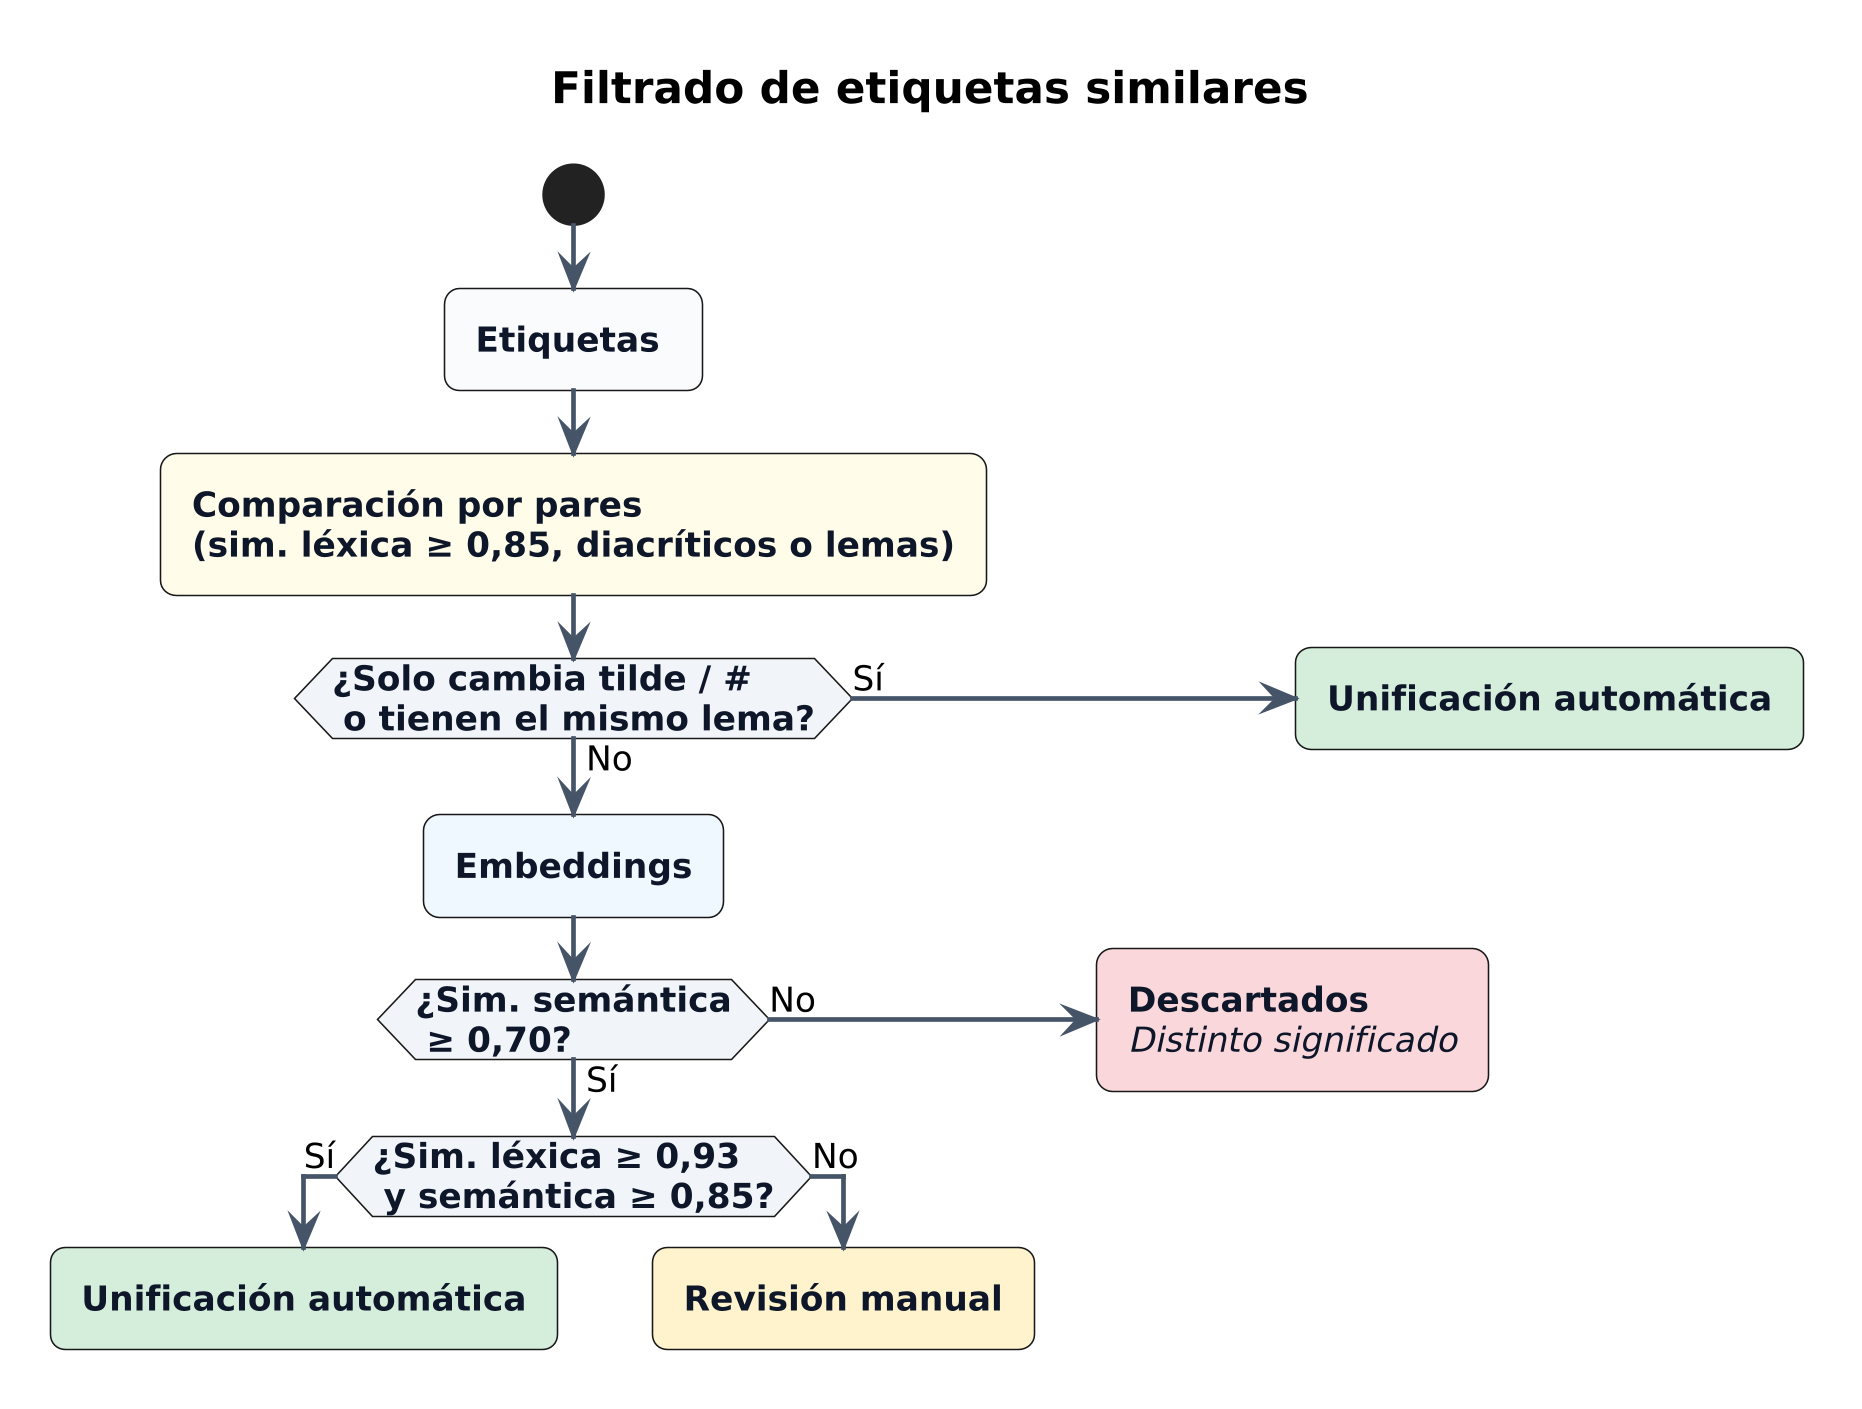
\includegraphics[width=0.65\linewidth]{../docs/UML/2.4.2.png}
\hfill
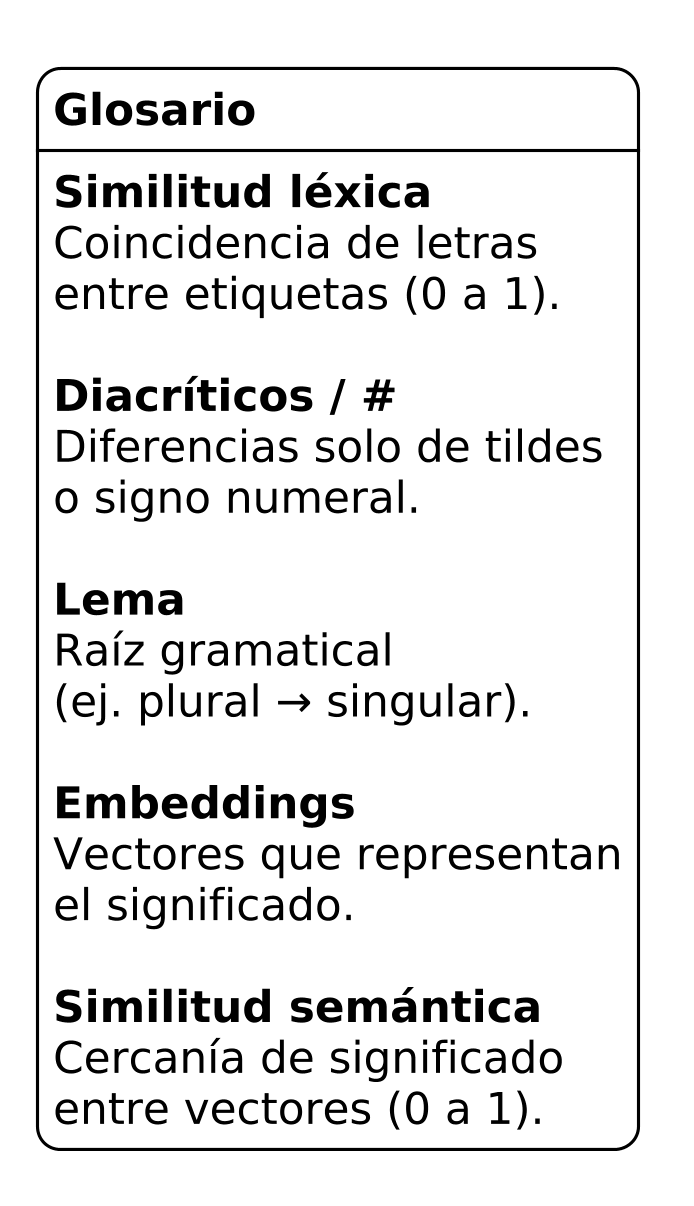
\includegraphics[width=0.28\linewidth]{../docs/UML/2.4.2-2.png}
\caption{Pipeline de filtrado morfológico y semántico de etiquetas}
\end{figure}

De los \textbf{51 pares} iniciales encontrados, el filtro descartó
\textbf{20} y dividió los \textbf{31 válidos} en dos grupos:

{\def\LTcaptype{none} % do not increment counter
\begin{longtable}[]{@{}
  >{\raggedright\arraybackslash}m{(\linewidth - 4\tabcolsep) * \real{0.3077}}
  >{\centering\arraybackslash}m{(\linewidth - 4\tabcolsep) * \real{0.3846}}
  >{\raggedright\arraybackslash}m{(\linewidth - 4\tabcolsep) * \real{0.3077}}@{}}
\toprule\noalign{}
\begin{minipage}[b]{\linewidth}\raggedright
Resultado
\end{minipage} & \begin{minipage}[b]{\linewidth}\centering
Cantidad de pares
\end{minipage} & \begin{minipage}[b]{\linewidth}\raggedright
Ejemplos detectados (\texttt{Variante} \(\rightarrow\)
\texttt{Canónico})
\end{minipage}\\ \midrule
\midrule\noalign{}
\endhead
\bottomrule\noalign{}
\endlastfoot
\textbf{Fusiones automáticas} & \textbf{26} & \emph{Mexico}
\(\rightarrow\) \emph{México}, \emph{Religion} \(\rightarrow\)
\emph{Religión}, \emph{Crisiis Climática} \(\rightarrow\) \emph{Crisis
Climática}, \emph{Gabrielboric} \(\rightarrow\) \emph{Gabriel Boric}\\ \midrule
\textbf{Revisión manual} & \textbf{5} & \emph{Arte} \(\rightarrow\)
\emph{Artes}, \emph{Neoliberalismo} \(\rightarrow\) \emph{Liberalismo},
\emph{Madres De Plaza De Mayo} \(\rightarrow\) \emph{Abuelas De Plaza De
Mayo}\\ \midrule
\end{longtable}
}

\subsubsection{2.5. Motor de recomendación de
artículos}\label{motor-de-recomendaciuxf3n-de-artuxedculos}

Se construyó un recomendador basado en los Tópicos encontrados, que
funciona en tres pasos:

\begin{enumerate}
\def\labelenumi{\arabic{enumi}.}
\item
  \textbf{Distribución de tópicos por nota:} En lugar de mirar
  únicamente el tópico mas cercano de cada artículo, se calculó un
  vector de probabilidades con el peso que tiene cada uno de los 23
  Tópicos (los 22 tópicos temáticos más el Tópico 100) dentro de cada
  nota, formando una matriz de \textbf{3.556 × 23}.
\item
  \textbf{Similitud coseno:} Al elegir un artículo de consulta, se toma
  su vector de 23 probabilidades y se calcula la similitud coseno contra
  los vectores de todos los demás artículos del archivo.
\item
  \textbf{Ranking de recomendaciones:} Se ordenan los artículos de mayor
  a menor similitud y se devuelven los más cercanos.
\end{enumerate}

\begin{figure}[H]
\centering
\pandocbounded{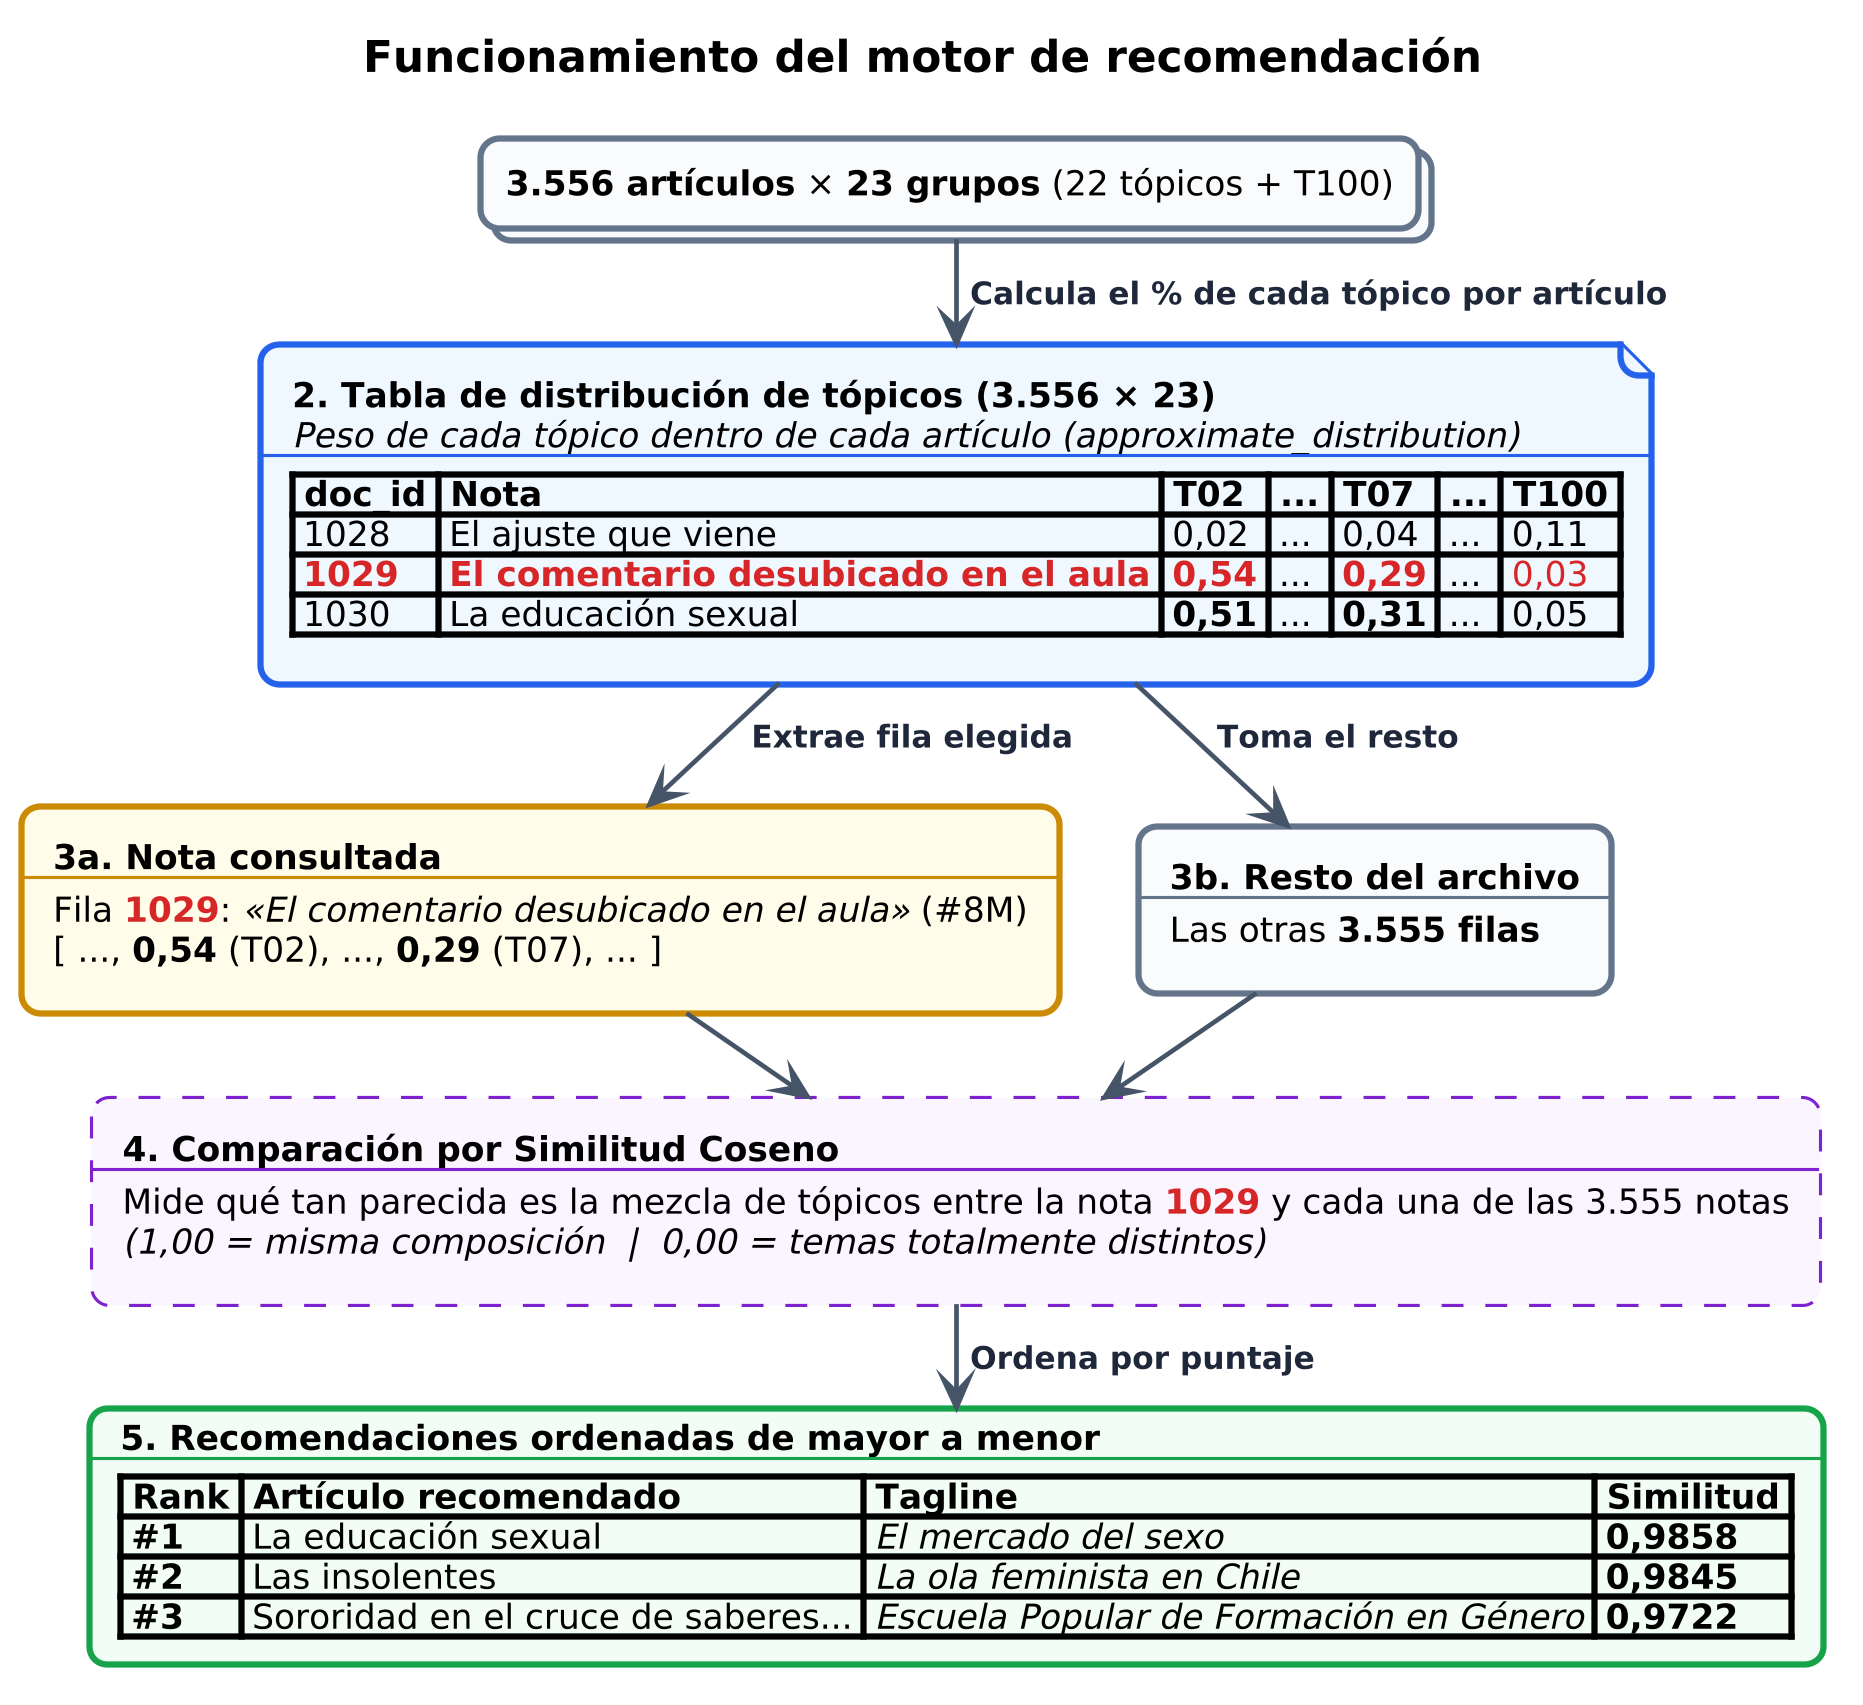
\includegraphics[keepaspectratio]{../docs/UML/2.5.1.png}}
\caption{Diagrama del motor de recomendación}
\end{figure}

\paragraph{\texorpdfstring{Caso de prueba en detalle: \emph{El
comentario desubicado en el
aula}}{Caso de prueba en detalle: El comentario desubicado en el aula}}\label{caso-de-prueba-en-detalle-el-comentario-desubicado-en-el-aula}

Para probar el funcionamiento del recomendador sobre una nota que no
esté tan dominada por un solo Tópico, se uso el artículo \emph{El
comentario desubicado en el aula}, cuyo tópico principal es \textbf{02}
(\texttt{feminismo\_feminista\_aborto}), pero que también tiene un peso
relevante en el tópico \textbf{07}
(\texttt{pedagógico\_enseñanza\_escolar}).

Al rankear por similitud, los primeros resultados hablan de
los mismos temas, incluso notas que habían quedado asignadas al
\textbf{Tópico 100} (\emph{La educación sexual} en primer lugar, con
similitud \texttt{0,9858}) o al \textbf{Tópico 07: pedagógico,
enseñanza, escolar} (\emph{Sororidad en el cruce de saberes populares y
académicos}, en tercer lugar):

% {\def\LTcaptype{none} % do not increment counter
% \begin{longtable}[]{@{}
%   >{\centering\arraybackslash}m{(\linewidth - 10\tabcolsep) * \real{0.1923}}
%   >{\raggedright\arraybackslash}m{(\linewidth - 10\tabcolsep) * \real{0.1538}}
%   >{\raggedright\arraybackslash}m{(\linewidth - 10\tabcolsep) * \real{0.1538}}
%   >{\raggedright\arraybackslash}m{(\linewidth - 10\tabcolsep) * \real{0.1538}}
%   >{\raggedright\arraybackslash}m{(\linewidth - 10\tabcolsep) * \real{0.1538}}
%   >{\centering\arraybackslash}m{(\linewidth - 10\tabcolsep) * \real{0.1923}}@{}}
% \toprule\noalign{}
% \begin{minipage}[b]{\linewidth}\centering
% Rank
% \end{minipage} & \begin{minipage}[b]{\linewidth}\raggedright
% Título
% \end{minipage} & \begin{minipage}[b]{\linewidth}\raggedright
% Tagline
% \end{minipage} & \begin{minipage}[b]{\linewidth}\raggedright
% Tópico dominante
% \end{minipage} & \begin{minipage}[b]{\linewidth}\raggedright
% Etiquetas
% \end{minipage} & \begin{minipage}[b]{\linewidth}\centering
% Similitud
% \end{minipage}\\ \midrule
% \midrule\noalign{}
% \endhead
% \bottomrule\noalign{}
% \endlastfoot
% 1 & \emph{La educación sexual} & El mercado del sexo &
% \texttt{100\_outliers\_miscelaneo} & Sin etiquetas & 0,9858\\ \midrule
% 2 & \emph{Las insolentes} & La ola feminista en Chile &
% \texttt{2\_feminismo\_feminista\_aborto} & Sin etiquetas & 0,9845\\ \midrule
% 3 & \emph{Sororidad en el cruce de saberes populares y académicos} &
% Escuela Popular de Formación en Género &
% \texttt{7\_pedagógico\_enseñanza\_escolar} & Feminismos; Territorio
% Educativo & 0,9722\\ \midrule
% 4 & \emph{Manual de instrucciones para hablar con E} & Lenguaje
% inclusivo & \texttt{100\_outliers\_miscelaneo} & Feminismos; Lenguaje
% inclusivo & 0,9722\\ \midrule
% 5 & \emph{``Mostramos lo que queremos, y que se jodan''} & Las pibas, la
% ropa, la escuela & \texttt{7\_pedagógico\_enseñanza\_escolar} & Sin
% etiquetas & 0,9709\\ \midrule
% \end{longtable}
% }
{\def\LTcaptype{none} % do not increment counter
\begin{longtable}[]{@{}
  >{\centering\arraybackslash}m{(\linewidth - 10\tabcolsep) * \real{0.0800}}
  >{\raggedright\arraybackslash}m{(\linewidth - 10\tabcolsep) * \real{0.2000}}
  >{\raggedright\arraybackslash}m{(\linewidth - 10\tabcolsep) * \real{0.1800}}
  >{\raggedright\arraybackslash}m{(\linewidth - 10\tabcolsep) * \real{0.2400}}
  >{\raggedright\arraybackslash}m{(\linewidth - 10\tabcolsep) * \real{0.1800}}
  >{\centering\arraybackslash}m{(\linewidth - 10\tabcolsep) * \real{0.1200}}@{}}
\toprule\noalign{}
\begin{minipage}[b]{\linewidth}\centering
Rank
\end{minipage} & \begin{minipage}[b]{\linewidth}\raggedright
Título
\end{minipage} & \begin{minipage}[b]{\linewidth}\raggedright
Tagline
\end{minipage} & \begin{minipage}[b]{\linewidth}\raggedright
Tópico dominante
\end{minipage} & \begin{minipage}[b]{\linewidth}\raggedright
Etiquetas
\end{minipage} & \begin{minipage}[b]{\linewidth}\centering
Similitud
\end{minipage} \\
\midrule\noalign{}
\endhead
\bottomrule\noalign{}
\endlastfoot
1 & \emph{La educación sexual} & El mercado del sexo &
\texttt{100\_\allowbreak outliers\_\allowbreak miscelaneo} & Sin etiquetas & 0,9858 \\ \midrule
2 & \emph{Las insolentes} & La ola feminista en Chile &
\texttt{2\_\allowbreak feminismo\_\allowbreak feminista\_\allowbreak aborto} & Sin etiquetas & 0,9845 \\ \midrule
3 & \emph{Sororidad en el cruce de saberes populares y académicos} &
Escuela Popular de Formación en Género &
\texttt{7\_\allowbreak pedagógico\_\allowbreak enseñanza\_\allowbreak escolar} & Feminismos; Territorio
Educativo & 0,9722 \\ \midrule
4 & \emph{Manual de instrucciones para hablar con E} & Lenguaje
inclusivo & \texttt{100\_\allowbreak outliers\_\allowbreak miscelaneo} & Feminismos; Lenguaje
inclusivo & 0,9722 \\ \midrule
5 & \emph{``Mostramos lo que queremos, y que se jodan''} & Las pibas, la
ropa, la escuela & \texttt{7\_\allowbreak pedagógico\_\allowbreak enseñanza\_\allowbreak escolar} & Sin
etiquetas & 0,9709 \\
\end{longtable}
}

En los mapas siguientes se observa la ubicación del artículo consultado
(diamante rojo) y sus 10 recomendaciones tanto en el \textbf{espacio de
\emph{embeddings}} como en el \textbf{espacio de probabilidades de
Tópicos} (proyecciones UMAP 2D):

\begin{figure}[H]
\centering
\pandocbounded{\includegraphics[keepaspectratio,alt={Ubicación en el
espacio de
embeddings}]{../outputs/figuras_informe/recomendador_mapa_embeddings.png}}
\caption{Ubicación en el espacio de embeddings}
\end{figure}

\begin{figure}[H]
\centering
\pandocbounded{\includegraphics[keepaspectratio,alt={Ubicación en el
espacio
temático}]{../outputs/figuras_informe/recomendador_mapa_tematico.png}}
\caption{Ubicación en el espacio temático}
\end{figure}

En el mapa por \emph{embeddings} las 10 recomendaciones (círculos
amarillos) se reparten en dos zonas distintas: la mayoría rodea al
artículo consultado (diamante rojo) dentro del área de
\textbf{\texttt{Tópico\ 2\_feminismo\_feminista\_aborto}}, mientras que
otro grupo aparece más arriba, dentro de
\textbf{\texttt{Tópico\ 7\_pedagógico\_enseñanza\_escolar}}. En cambio,
al proyectar el espacio de distribución de tópicos ---que es el que
utiliza el recomendador---, todos los artículos sugeridos quedan
agrupados de forma compacta junto al artículo original, exactamente en
la zona de transición entre ambos núcleos temáticos. Esto muestra cómo
el sistema puede recomendar notas que semánticamente están en regiones
diferentes pero que hablen de los mismos temas.

Finalmente, se contrasta la distribución de Tópicos del artículo
consultado frente a la recomendación \textbf{\#1} y la \textbf{\#10}, se
verifica cómo se preservan los tópicos principales en el primero y
comienza a variar gradualmente en los tópicos secundarios en el décimo:

\begin{figure}[H]
\centering
\pandocbounded{\includegraphics[keepaspectratio,alt={Comparación con la
recomendación
\#1}]{../outputs/figuras_informe/recomendador_composicion_topicos_rec1.png}}
\caption{Comparación con la recomendación \#1}
\end{figure}

\begin{quote}
\small\textbf{Nota:} El tópico dominante y el gráfico de distribución provienen de dos cálculos distintos: 
mientras que el tópico dominante se define por cercanía en el espacio de embeddings (donde \emph{La educación sexual} 
no alcanzo el umbral de $0,65$ con ninguno y cayó en el \texttt{Tópico 100}), el vector de distribución
utilizado por el recomendador estima el peso de cada tema a partir de las palabras clave (c-TF-IDF) de cada grupo. 
Por eso el artículo no tiene como mayor nivel de la distribución el Tópico 100, se refieren a cosas diferentes.
\end{quote}

\begin{figure}[H]
\centering
\pandocbounded{\includegraphics[keepaspectratio,alt={Comparación con la
recomendación
\#10}]{../outputs/figuras_informe/recomendador_composicion_topicos_rec10.png}}
\caption{Comparación con la recomendación \#10}
\end{figure}

\subsubsection{2.6. Aplicación web interactiva
(Streamlit)}\label{aplicaciuxf3n-web-interactiva-streamlit}

De forma complementaria al análisis, se desarrolló y desplegó un informe
interactivo en \textbf{Streamlit}
(\href{https://anfibia-informe-1.streamlit.app/}{anfibia-informe-1.streamlit.app})
para que el equipo editorial de \emph{Revista Anfibia} pueda explorar
los resultados sin ejecutar código (la aplicación se apoya sobre un
repositorio oculto que contiene únicamente metadatos agregados, matrices
numéricas y gráficos exportados):

\begin{enumerate}
\def\labelenumi{\arabic{enumi}.}
\item
  \textbf{Análisis de los artículos:} Exploración de las palabras, las
  categorías editoriales y su evolución año a año.
\item
  \textbf{Creación y exploración de tópicos:} Visualización interactiva
  de los tópicos descubiertos y su comportamiento en el tiempo.
\item
  \textbf{Auditoría de etiquetas:} Cruce de etiquetas frente a
  categorías y tópicos, junto con tablas interactivas de propuestas de
  normalización (fusiones automáticas, revisión manual, etc).
\item
  \textbf{Recomendación de artículos:} Búsqueda de notas por título o
  identificador para obtener artículos similares mediante similitud del
  coseno y visualizarlos en el mapa UMAP 2D.
\end{enumerate}

Cabe aclarar que esta versión desplegada funciona sobre una
\textbf{iteración previa del modelo de tópicos} y del proyecto en
general, por lo que actúa como un prototipo de validación.

\subsection{3. Conclusiones y Líneas
Futuras}\label{conclusiones-y-luxedneas-futuras}

\begin{enumerate}
\def\labelenumi{\arabic{enumi}.}
\item
  \textbf{Tópicos:} Desde los primeros modelos hasta el final, se redujo
  la proporción de artículos sin tópico asignado del \textbf{35,1 \% al
  15,0 \%} (534 notas reunidas en el \textbf{Tópico 100}). El
  \textbf{85,0 \%} restante quedó organizado en \textbf{22 tópicos bien
  definidos}, que reflejan los principales ejes de la revista (política,
  literatura, feminismos, justicia, economía, etc.). A futuro, queda
  pendiente seguir refinando los tópicos y analizar qué efecto tiene
  incluir el \textbf{Tópico 100} en el cálculo de las distribuciones y
  en los análisis posteriores.
\item
  \textbf{Etiquetado:} Todavía hay muchos artículos sin etiquetar y una
  fragmentación muy alta. Aunque en este proyecto se probaron formas
  concretas de limpiarlas y agruparlas, hace falta más trabajo y definir
  criterios claros junto a \emph{Revista Anfibia}.
\item
  \textbf{Recomendación:} Se logró recomendar notas relacionadas
  mediante sus distribuciones de tópicos aunque su tópico principal sea
  distinto, incluso cuando cayeron en el \textbf{Tópico 100}. También se
  evaluó sumar la similitud directa entre los \emph{embeddings} de los
  textos para complementar el cálculo, pero se dejó de lado por no tener
  todavía una métrica objetiva para evaluar qué tan buena es cada
  recomendación; como idea, se plantea usar modelos de lenguaje (LLMs)
  para crear esta métrica.
\end{enumerate}

Aparte de las mejoras del trabajo realizado, queda pensar en la
integración en la página web de \emph{Revista Anfibia}. Eso tendrá que
esperar a que lo demás esté completamente definido como prototipo;
luego, mediante la elaboración de una API (o alguna otra alternativa,
todavía no definida), deberá integrarse a la web.

\subsection{4. Aprendizajes}\label{aprendizajes}

Este proyecto permitió poner en práctica herramientas y conceptos
centrales de la Ciencia de Datos sobre un caso de estudio real:

\begin{itemize}
\item
  \textbf{Datos y gobernanza:} Trabajar con datos reales de una página
  web permitió dimensionar la importancia de la limpieza, el filtrado y
  la aplicación de criterios estrictos de privacidad para lo que se
  muestra de manera pública y antes de entrenar cualquier modelo.
\item
  \textbf{NLP aplicado:} La lematización con spaCy, el diseño de
  stopwords y la experimentación con BERTopic, UMAP y HDBSCAN fueron
  herramientas personalmente nunca antes usadas, que requieren un ajuste
  fino constante, control y validación métrica y visual. Todo esto se
  comprendió en profundidad al elaborar el proyecto.
\item
  \textbf{Trabajo interdisciplinario:} La interacción con el equipo de
  \emph{Revista Anfibia} marcó la necesidad de una comunicación
  constante. Por ejemplo, respecto a las etiquetas, estas respondían a
  decisiones editoriales específicas, por lo cual no se podía
  simplemente borrarlas o cambiarlas de forma automatizada sin consultar
  lo que opinaban.
\end{itemize}

\begin{center}\rule{0.5\linewidth}{0.5pt}\end{center}

\subsection{Anexo: Algunos conceptos}\label{anexo-algunos-conceptos}

Son conceptos que atraviesan varias partes del informe de diferentes
maneras.

\subsubsection{\texorpdfstring{A.1.
\emph{Embeddings}}{A.1. Embeddings}}\label{a.1.-embeddings}

Un \textbf{\emph{embedding}} transforma una palabra, frase o artículo
completo (texto en general) en un vector numérico de tamaño fijo (en
este trabajo, de \textbf{384 dimensiones} generadas con
\texttt{paraphrase-multilingual-MiniLM-L12-v2}).

Cada una de esas dimensiones captura rasgos latentes del significado y
del contexto en el que aparecen las palabras, de modo que textos con
sentido similar tendrán vectores similares.

Ejemplo con \texttt{paraphrase-multilingual-MiniLM-L12-v2}:

\[\text{``crisis económica''} \longrightarrow [-0.02, -0.13, -0.03, \dots, -0.26] \in \mathbb{R}^{384}\]
\[\text{``caída del salario''} \longrightarrow [-0.15, 0.19, 0.05, \dots, 0.12] \in \mathbb{R}^{384}\]
\[\text{``partido de fútbol''} \longrightarrow [0.04, 0.22, -0.26, \dots, -0.02] \in \mathbb{R}^{384}\]

\subsubsection{A.2. Centroide}\label{a.2.-centroide}

Cuando cada artículo o palabra se representa como un vector numérico (ya
sea un \emph{embedding} o una distribución de tópicos), el
\textbf{centroide} de un grupo es simplemente el promedio de todos los
vectores que lo integran:

\[\vec{C} = \frac{1}{N} \sum_{i=1}^{N} \vec{v}_i\]

Donde \(N\) es la cantidad de artículos del grupo y \(\vec{v}_i\) el
vector de cada uno. Geométricamente representa el ``punto medio'' del
conjunto, y se utilizó en el trabajo para:

\begin{itemize}
\item
  \textbf{Representación de tópicos :} Identificar las palabras clave
  más cercanas al centroide de cada tópico.
\item
  \textbf{Artículos representativos:} Encontrar qué nota está más cerca
  del centro de cada tópico o de un pico temporal dentro de esa ventana
  de tiempo.
\item
  \textbf{Reasignación de \emph{outliers}:} Medir qué tan cerca estaba
  cada artículo \texttt{-1} del centro de los tópicos existentes y
  asignarlo al mas cercano (siempre que pasara el umbral).
\end{itemize}

\begin{figure}[H]
\centering
\pandocbounded{\includegraphics[keepaspectratio,alt={Representación
geométrica del
centroide}]{../outputs/figuras_informe/anexo_centroide.png}}
\caption{Representación geométrica del centroide}
\end{figure}

\subsubsection{A.3. Similitud y distancia
coseno}\label{a.3.-similitud-y-distancia-coseno}

La similitud del coseno mide qué tan parecidos son dos vectores mirando
el \textbf{ángulo} que forman entre sí, sin importar su magnitud:

\[\text{Sim}(\vec{A}, \vec{B}) = \frac{\vec{A} \cdot \vec{B}}{\|\vec{A}\| \, \|\vec{B}\|}\]

El resultado varía entre \textbf{0} y \textbf{1} para frecuencias o
probabilidades (o entre \textbf{-1} y \textbf{1} en \emph{embeddings}):

\begin{itemize}
\item
  \textbf{Cercano a \texttt{1}:} Ambos vectores apuntan en la misma
  dirección (significado muy similar).
\item
  \textbf{Cercano a \texttt{0}:} Son perpendiculares entre sí (no
  comparten relación).
\end{itemize}

\begin{figure}[H]
\centering
\pandocbounded{\includegraphics[keepaspectratio,alt={Representación
geométrica de la similitud del
coseno}]{../outputs/figuras_informe/anexo_similitud_coseno.png}}
\caption{Representación geométrica de la similitud del coseno}
\end{figure}

A partir de esta medida se define también la \textbf{distancia del
coseno} (las proyecciones UMAP y en los dendrogramas), que simplemente
invierte:

\[\text{Dist}(\vec{A}, \vec{B}) = 1 - \text{Sim}(\vec{A}, \vec{B})\]

De este modo, cuando dos vectores son idénticos en dirección
(\(\text{Sim} = 1\)), su distancia es \textbf{\texttt{0}}, y a medida
que divergen, la distancia aumenta.

\end{document}
